% Memory Agent Security: Unified Attack Evaluation and Defense Framework
%
% Compilation: pdflatex main.tex && bibtex main && pdflatex main.tex && pdflatex main.tex
% Or use latexmk: latexmk -pdf main.tex

\documentclass[10pt]{article}

% --- packages ---
\usepackage[margin=1in]{geometry}
\usepackage{amsmath, amssymb, amsthm}
\usepackage{graphicx}
\usepackage{booktabs}
\usepackage{xcolor}
\usepackage{hyperref}
\usepackage{natbib}
\usepackage{subcaption}
\usepackage{microtype}
\usepackage{tikz}
\usetikzlibrary{arrows.meta, positioning, shapes.geometric, fit, backgrounds, patterns}

% --- figure path (all generated figures live in figures/) ---
\graphicspath{{figures/}}

% --- theorem environments ---
\newtheorem{theorem}{Theorem}
\newtheorem{lemma}{Lemma}
\newtheorem{proposition}{Proposition}
\newtheorem{definition}{Definition}
\newtheorem{remark}{Remark}

% --- custom macros ---
\newcommand{\asrr}{\text{ASR-R}}
\newcommand{\asra}{\text{ASR-A}}
\newcommand{\asrt}{\text{ASR-T}}
\newcommand{\isr}{\text{ISR}}
\newcommand{\tpr}{\text{TPR}}
\newcommand{\fpr}{\text{FPR}}
\newcommand{\EE}{\mathbb{E}}
\newcommand{\RR}{\mathbb{R}}
\newcommand{\sad}{\textsc{SAD}}
\newcommand{\agentpoison}{\textsc{AgentPoison}}
\newcommand{\minja}{\textsc{MINJA}}
\newcommand{\injecmem}{\textsc{InjecMEM}}
\newcommand{\trigger}{T}
\newcommand{\passage}{p_{\mathrm{adv}}}
\newcommand{\enc}{E}

\title{%
  \textbf{Poisoning the Memory: A Unified Framework for Attacking and\\
  Defending LLM Agent Memory Systems}
}

\author{%
  Ishrith Gowda\\
  University of California, Berkeley\\
  \texttt{ishrithgowda@berkeley.edu}
}

\date{March 2026}

\begin{document}

\maketitle

\begin{abstract}
LLM agents increasingly rely on external memory systems to persist context
across sessions.  We show that this memory constitutes a critical and largely
undefended attack surface.  We present a unified evaluation framework for
three recently proposed memory poisoning attacks---\agentpoison{}
\citep{chen2024agentpoison}, \minja{} \citep{dong2025minja}, and
\injecmem{} \citep{injecmem2026}---implemented over a realistic FAISS-backed
vector memory store (all-MiniLM-L6-v2, 384-dim) with a 200-entry synthetic
agent memory corpus.

We identify and correct a systematic evaluation error in prior simulations:
\agentpoison{}'s attack success rate at retrieval (\asrr) was underestimated
because victim queries were issued \emph{without} the attacker-controlled
trigger token at evaluation time.  The paper's evaluation protocol
(Chen et al., Algorithm~2) prepends the trigger to every query;
with this correction and a centroid-targeting adversarial passage,
\asrr{} increases from 0.25 to 1.00 at 2.4\% poison rate.

On the defense side, we propose \sad{}---a Semantic Anomaly Detection
defense that flags adversarial memory entries by their anomalously high
cosine similarity to observed victim queries.  We evaluate all five defenses
(Watermark, Validation, Proactive, Composite, \sad{}) in a pre-ingestion
filtering model across a full $3 \times 5$ attack-defense interaction matrix.
We find that no single defense is uniformly effective, motivating composite
defense portfolios.  For \sad{} specifically, we identify a fundamental gradient tension for
continuous adversaries: any perturbation that reduces the anomaly score
also reduces retrieval rank via the shared cosine similarity objective.
Empirically, word-level synonym substitution circumvents this tension
because semantic embeddings are synonym-invariant: synonym replacements
achieve evasion rates $\geq 0.80$ with $\Delta\asrr \approx 0$, motivating
defenses that incorporate lexical diversity features.
We further show that \sad{} calibrated on \emph{triggered} victim queries
achieves $\tpr = 1.00$, $\fpr = 0.00$ for \agentpoison{}---closing the blind
spot that arises under plain-query calibration.

We additionally implement three paper-faithful extensions: (i) DPR HotFlip
gradient-guided trigger optimization~\citep{ebrahimi2018hotflip} over the
\texttt{facebook/dpr-ctx\_encoder-single-nq-base} (768-dim), improving mean
triggered-query similarity from 0.71 to 0.78; (ii) the full token-level
unigram watermark~\citep{zhao2024watermark} via a GPT-2 backbone, achieving
$83\%$ higher z-scores than character-level at short text lengths; and
(iii) a local GPT-2 agent evaluator providing a directly measured lower bound
on $\asra$ ($0.42$--$0.51$ across attacks) that confirms the modelled values
are conservative.

We extend the evaluation across three further dimensions.
\emph{Multi-encoder transferability}: we evaluate all three attacks and
\sad{} across seven retrieval encoders (MiniLM-L6, MPNet-Base, E5-base,
Contriever, BGE-large, OpenAI text-embedding-3-small/-large) and compute
linear Centered Kernel Alignment (CKA) across all encoder pairs, finding
that high inter-encoder CKA predicts cross-encoder ASR-R transferability.
\emph{Multi-agent epidemic propagation}: a discrete-step SIR model over a
shared FAISS knowledge base shows that a single poisoned entry spreads to
connected agents via re-storage; \sad{}-based write-time quarantine halts
secondary infection by blocking flagged entries before they are re-stored.
\emph{Graph-structured memory}: we extend the threat model to GraphRAG-style
entity-relation stores, implementing hub insertion, edge-hijack, and
subgraph-cluster attacks that exploit graph topology, and two graph-native
defenses---degree-anomaly detection and adjacency contamination
scoring---that identify structurally anomalous nodes without requiring
labeled poison examples.
Production-scale \asra{} is directly measured using a GPT-4o-mini agent
evaluator (OpenAI \texttt{text-embedding-3-large} retrieval, $T=0$),
and FPR for all defenses is validated over 20 independent trials using
Clopper-Pearson exact binomial confidence intervals, confirming
FPR\,$=0.000$ for watermark and \sad{} combined-mode at $95\%$ confidence.

All code, experiments, and figures are open-sourced at
\url{https://github.com/ishrith-gowda/memory-agent-security}.
\end{abstract}

% section files
\section{Introduction}
\label{sec:intro}

% --- motivation ---
Modern LLM agents persist context across sessions through external memory
systems such as Mem0~\citep{mem0}, A-MEM~\citep{amem}, and
MemGPT~\citep{memgpt2023}.  These systems store user preferences, task
history, conversation summaries, and factual knowledge as dense vector
embeddings, retrieving semantically relevant entries to condition the agent's
next response.  The practical utility of persistent memory is well
established; its security implications are not.

% --- the attack surface ---
An adversary who can influence the contents of an agent's memory---whether
through direct write access, crafted user interaction, or exploitation of
the agent's self-storage mechanism---can covertly redirect agent behavior
across arbitrary future sessions.  Unlike jailbreaks, which operate on a
single interaction, memory poisoning attacks \emph{persist}: a single
adversarial entry may remain in memory for weeks and trigger on every
related query.  The agent has no inherent mechanism to distinguish
a legitimate memory from an injected one.

% --- three attacks ---
Three recent papers have characterized different threat models for memory
poisoning.  \agentpoison{} \citep{chen2024agentpoison} requires write access
to the memory/knowledge base and optimizes a short trigger token sequence
such that any user query containing the trigger retrieves the adversarial
entry with high probability.  \minja{} \citep{dong2025minja} requires no
memory access: the attacker poses as a regular user and submits crafted
queries that cause the agent to auto-generate and store adversarial reasoning
chains.  \injecmem{} \citep{injecmem2026} achieves injection in a single
interaction via a ``retriever-agnostic anchor'' passage designed to
match many query types simultaneously.

% --- our contributions ---
This paper makes six contributions:

\begin{enumerate}
  \item \textbf{Unified evaluation framework.}  We implement all three attacks
  over a realistic FAISS-backed vector memory system with a 200-entry synthetic
  agent corpus and three paper-faithful success metrics: $\asrr$ (retrieval
  success rate), $\asra$ (action execution rate given retrieval), and $\asrt$
  (end-to-end task hijacking rate) as defined in \citet{chen2024agentpoison}.

  \item \textbf{Evaluation protocol correction.}  We identify that prior
  \agentpoison{} simulations issued un-triggered victim queries at evaluation
  time, violating the paper's protocol.  With the correct triggered-query
  evaluation and a centroid-targeting adversarial passage, $\asrr$ increases
  from 0.25 to 1.00 (Section~\ref{sec:experiments}).

  \item \textbf{Semantic Anomaly Detection (\sad{}).}  We propose a novel
  defense that detects adversarial memory entries by their anomalously high
  cosine similarity to observed victim queries, without requiring labeled
  attack examples.  Under plain-query calibration, \sad{} achieves
  $\tpr=1.00$, $\fpr\approx0.05$ for \minja{} and $\tpr=0.20$ for \injecmem{};
  calibrating on triggered queries closes the \agentpoison{} blind spot
  ($\tpr=0.00 \to 1.00$, $\fpr=0.00$, threshold shift $0.482 \to 0.432$).
  We prove (Proposition~\ref{prop:gradient_tension}) that continuous
  evasion in embedding space is impossible; the empirical synonym-invariance
  loophole for discrete substitution is characterised in Remark~\ref{rem:synonym}.

  \item \textbf{Full attack-defense interaction matrix.}  We evaluate all
  $3 \times 5$ (attack, defense) pairs under a pre-ingestion filtering model,
  revealing that no single defense dominates uniformly and motivating composite
  defense portfolios.

  \item \textbf{Adaptive adversary analysis.}  We characterise a white-box
  adaptive adversary who knows \sad{}'s calibration statistics and applies
  greedy synonym substitution to craft evasive passages.
  Proposition~\ref{prop:gradient_tension} proves that in continuous
  embedding space any reduction in anomaly score simultaneously reduces
  retrieval rank (shared cosine gradient).  Remark~\ref{rem:synonym}
  identifies the discrete loophole: synonym-invariant encoders make
  word-level substitution effectively free ($\Delta\asrr \approx 0$,
  evasion $\geq 0.80$), revealing that lexical diversity features are
  needed to close this gap.

  \item \textbf{Paper-faithful implementations and measured bounds.}  We
  implement DPR HotFlip gradient-guided trigger optimization
  (improving mean triggered-query cosine similarity from 0.71 to 0.78),
  the full token-level unigram watermark \citep{zhao2024watermark} via a
  GPT-2 backbone ($p_{\text{green}} \approx 0.711$, $+83\%$ z-score at
  short texts), and a local GPT-2 agent evaluator providing directly measured
  lower bounds on $\asra$ (0.42--0.51 across attacks vs.\  modelled
  upper bounds of 0.68--0.76).
\end{enumerate}

% --- paper organization ---
Section~\ref{sec:related} reviews related work.
Section~\ref{sec:threat} formalizes the threat model.
Sections~\ref{sec:attacks} and~\ref{sec:defenses} describe attack and defense
implementations.  Section~\ref{sec:experiments} reports empirical results.
Section~\ref{sec:discussion} discusses limitations and future work.

\section{Related Work}
\label{sec:related}

\paragraph{Memory poisoning attacks on LLM agents.}
\citet{chen2024agentpoison} introduce \agentpoison{}, the first attack to
exploit the retrieval mechanism of LLM agent memory systems.  They formulate
trigger optimization as a constrained gradient problem over the embedding
space of a dense retriever (DPR~\citep{karpukhin2020dense}) and demonstrate
attacks on three production agent frameworks (LangChain, Voyager, ReAct),
achieving $\asrr \geq 0.80$ at below 0.1\% poison rate.
\citet{dong2025minja} extend the threat model to a \emph{query-only} setting:
the attacker has no direct memory access and relies on the agent's auto-storage
of adversarial reasoning chains.  Their progressive-shortening indication
protocol achieves ISR of 98.2\% across three experimental platforms.
\citet{injecmem2026} propose a retriever-agnostic anchor strategy that achieves
broad recall via topic-covering passages designed to match many query types,
enabling injection in a single interaction.
\citet{memorygraft2025} demonstrate that successful experiences stored in
agent memory can be \emph{grafted}: an attacker implants a malicious
``experience record'' that is later retrieved and replicated as a legitimate
agent action, exploiting the union retrieval over lexical and embedding similarity.
Concurrent work on tool-use manipulation~\citep{yang2024watch} shows that
similar poisoning strategies transfer to agent tool selection, broadening
the attack surface beyond memory retrieval.
\citet{li2026memorypoisoning} provide an empirical comparison of memory
poisoning attacks and defenses in EHR agents, confirming that attack
effectiveness is largely robust to corpus size---consistent with our
corpus-size ablation (Appendix~\ref{sec:ablation_appendix}).

\paragraph{RAG corpus poisoning.}
Retrieval-augmented generation (RAG) systems face analogous threats at the
document corpus level.  \citet{zou2024poisonedrag} demonstrate that
adversarial documents optimized via HotFlip~\citep{ebrahimi2018hotflip}
can force specific LLM outputs when retrieved, achieving $> 90\%$ ASR
at million-scale knowledge bases.  \citet{chaudhari2024phantom}
construct phantom documents that match specific queries while appearing
semantically benign to human inspection.  \citet{xue2024badrag} show
that a small number of adversarially crafted documents can redirect LLM
answers across entire topic domains, consistent with our corpus-size ablation.
\citet{arzanipour2025ragsecurity} provide the first formal threat model
for RAG systems, defining adversary access tiers and formally bounding
the attack surface at the document and embedding levels.
\citet{tan2025revprag} detect poisoned RAG responses via LLM activation
analysis (ResNet18 on multi-layer activations), achieving $98\%$ TPR at
$1\%$ FPR---a complementary detection signal to our query-similarity approach.
Our work differs from RAG poisoning in that the adversarial entries are
\emph{agent-generated, semantically coherent memories} rather than external
documents, the threat persists across sessions without further adversarial
interaction, and defenses must operate at write time without full corpus visibility.

\paragraph{Backdoor attacks on neural retrieval.}
Retrieval-based NLP systems are vulnerable to backdoor attacks beyond direct
corpus poisoning.  \citet{yang2021rethinking} and \citet{carlini2024poisoning}
demonstrate that embedding-space backdoors can cause targeted retrievals
in open-domain question answering systems.  \citet{badchain2024} show that
chain-of-thought reasoning prompts can be backdoored, causing models to
follow malicious reasoning chains when a trigger phrase appears---analogous
to \minja{}'s bridging-step mechanism.
The ASB benchmark \citep{zhang2024asb} provides a unified evaluation
framework for backdoor attacks and defenses in classification settings;
we adapt its matrix format to the memory-agent threat model.
Neural Cleanse \citep{wang2019neuralcleanse} and STRIP \citep{gao2019strip}
are representative detection methods that inspired our proactive and composite
defense designs.  However, these methods are fundamentally model-centric:
Neural Cleanse requires white-box model access and reverse-engineers trigger
patterns in parameter space; STRIP perturbs \emph{inference-time inputs} and
detects Trojan activation via entropy collapse.  Neither applies to the
memory-poisoning setting: our defenses target raw \emph{stored content}
rather than model weights or inference activations, and must operate at
write time without access to the retrieval model's internal states.
This architectural difference motivates SAD's calibration-based approach,
which detects anomalous \emph{similarity} rather than anomalous \emph{activation}.

\paragraph{LLM watermarking for content provenance.}
\citet{zhao2024watermark} propose a provably robust token-level watermark
for LLM-generated text based on a green/red vocabulary partition, achieving
AUROC $> 0.97$ and providing formal guarantees under $\ell_\infty$-bounded
paraphrasing.  \citet{kirchenbauer2023watermark} independently develop
a similar scheme (KGW) and analyze its robustness to paraphrasing attacks.
\citet{hu2023unbiased} propose an unbiased watermarking scheme that avoids
the quality degradation associated with hard vocabulary partitions.
We adapt the Zhao et al.\ unigram scheme to character-level memory entries
that do not pass through a generative model (Section~\ref{sec:defenses});
our evasion evaluation mirrors the paraphrasing and dilution attacks studied
in \citet{kirchenbauer2023watermark} and extends them to copy-paste dilution
and adaptive vocabulary substitution.

\paragraph{Prompt injection and indirect injection attacks.}
\citet{perez2022ignore} first characterize prompt injection attacks, where
a crafted user input overrides system instructions.  \citet{greshake2023not}
extend this to \emph{indirect prompt injection}: adversarial content in
retrieved documents (web pages, emails, tool outputs) hijacks the agent's
behavior without the user's knowledge.  Memory poisoning is orthogonal:
the adversarial content is stored silently and triggers on future queries
without further adversarial interaction, persisting across sessions.
This makes memory poisoning strictly more dangerous in multi-session
deployments: a single poisoning event affects \emph{all} future interactions.

\paragraph{LLM agent security and memory systems.}
The LLM agent security landscape has broadened rapidly.
\citet{memgpt2023} introduce MemGPT's hierarchical memory system, which
our framework targets via the Mem0~\citep{mem0} and A-MEM~\citep{amem}
wrappers.  \citet{touvron2023llama} and \citet{openai2023gpt4} describe
production-scale LLMs that underpin modern agent deployments.
\citet{yang2024watch} identify that agent tool selection and memory retrieval
share a common embedding-based vulnerability; our attack-defense matrix
provides the first systematic cross-attack coverage in this setting.
\citet{gu2019badnets} establish the foundational backdoor threat model
that underlies our definition of memory poisoning (Definition~1).
\citet{zhang2024asb} benchmark 10 prompt injection attacks, memory poisoning,
and 11 defenses across 13 LLM backbones in the ASB framework; we adopt
its matrix format and extend coverage to pre-ingestion filtering defenses.
\citet{amemguard2025} propose a proactive defense combining consensus-based
validation over multiple memory retrievals with a ``lessons learned'' store;
their 95\% ASR reduction is complementary to our write-time filtering approach.

\paragraph{Anomaly detection for adversarial inputs.}
Our \sad{} defense draws on a line of anomaly detection work in NLP.
\citet{gao2019strip} use input perturbation to detect Trojan-activated
predictions; we adapt the key insight---that adversarial inputs cluster
differently from benign ones in representation space---to the memory entry
setting.  \citet{goldblum2022dataset} and \citet{hayase2021spectre} develop
spectral methods for detecting poisoned samples in supervised learning;
their methods require a labeled set of both clean and poisoned training examples
to compute a covariance structure and identify poisoned directions.
In the memory-agent setting, no labeled poison examples are available at
detection time, making spectral methods inapplicable.
\sad{} sidesteps this by exploiting the \emph{query-similarity signal}:
poison entries must be semantically close to victim queries (by attack
design), while benign entries are not, enabling calibration from benign
content alone.  \citet{lee2018simple} show that Mahalanobis distance to
class centroids is an effective out-of-distribution detector;
our cosine similarity threshold is the retrieval-space analogue, adapted
to the unsupervised, query-conditioned memory setting.

\input{sections/threat_model}
\section{Attack Implementations}
\label{sec:attacks}

\subsection{AgentPoison}

\agentpoison{} \citep{chen2024agentpoison} optimizes a trigger sequence
$\trigger^* = (t_1, \ldots, t_\ell)$ such that for any victim query
$q \in \mathcal{Q}_v$, the triggered embedding $E(q \oplus \trigger)$ is
close to the adversarial passage embedding $E(\passage)$:
\begin{equation}
  \trigger^* = \arg\max_\trigger\; \EE_{q \sim \mathcal{Q}_v}
  \left[\cos\!\left(E(q \oplus \trigger),\, E(\passage)\right)\right].
  \label{eq:agentpoison_obj}
\end{equation}

\paragraph{DPR HotFlip trigger optimization.}
We implement the paper-faithful gradient-guided trigger optimizer using the
DPR context encoder (\texttt{facebook/dpr-ctx\_encoder-single-nq-base},
768-dim BERT-based).  At each iteration, the gradient of the cosine-similarity
loss with respect to the trigger token embedding at position $i$ is computed:
\begin{equation}
  t_i^* = \arg\max_{v \in \mathcal{V}}\;
  \nabla_{e_{t_i}} \mathcal{L} \cdot e_v,
  \label{eq:hotflip}
\end{equation}
where $\mathcal{V}$ is the filtered BERT vocabulary (alphabetic, non-subword
tokens, $|\mathcal{V}| \approx 18{,}000$) and $e_v$ is the embedding of token
$v$.  Top-$n_{\text{cand}}=32$ candidates are evaluated with exact forward
passes; a GPT-2 perplexity gate ($\mathrm{ppl} < 500$) ensures trigger
fluency.  Figure~\ref{fig:dpr_convergence} shows convergence.

\paragraph{Centroid passage.}
The adversarial passage is built to target the centroid of victim query
embeddings:
\begin{equation}
  \passage = \mathrm{CentroidPassage}(\mathcal{Q}_v)
  = \text{passage covering vocabulary}\; \bigcup_{q \in \mathcal{Q}_v} \mathrm{KeyTerms}(q).
  \label{eq:centroid}
\end{equation}
$\mathrm{KeyTerms}$ extracts content words (stopword-filtered, frequency-ranked).
This places $\passage$ near the centroid of victim query embeddings, achieving
moderate-to-high cosine similarity with \emph{every} victim query.
The centroid passage plus DPR-optimized trigger achieves mean cosine
similarity 0.78 vs.\ 0.48 baseline (random trigger) and 0.71 (centroid only).

\paragraph{Triggered-query evaluation.}
A critical evaluation detail: the attacker controls query content at test
time (e.g., via a shared trigger deployed to compromised clients).  The
correct evaluation protocol (Chen et al., Algorithm~2) issues triggered
queries $q \oplus \trigger$, not plain queries $q$.  We correct this in our
framework and discuss the resulting performance improvement in
Section~\ref{sec:experiments}.

\paragraph{$\asra$ measurement.}
Beyond modelled $\asra$ (calibrated to paper-reported values,
$\mathcal{N}(0.68, 0.06^2)$), we provide a direct measurement via a local
GPT-2 agent evaluator (\textsc{LocalAgentEvaluator}): retrieved memory
entries are embedded in an agent prompt, GPT-2 generates a response, and
adversarial action execution is detected via keyword matching combined with a
perplexity gate ($\mathrm{ppl} < 200$) that rejects incoherent outputs.
GPT-2 acts as a tractable lower bound on true $\asra$; production LLMs
(GPT-4, Llama-3) are expected to achieve values at or above the modelled
upper bound (Section~\ref{sec:phase17_results}).

\IfFileExists{figures/fig_p17_dpr_convergence.pdf}{%
\begin{figure}[ht]
  \centering
  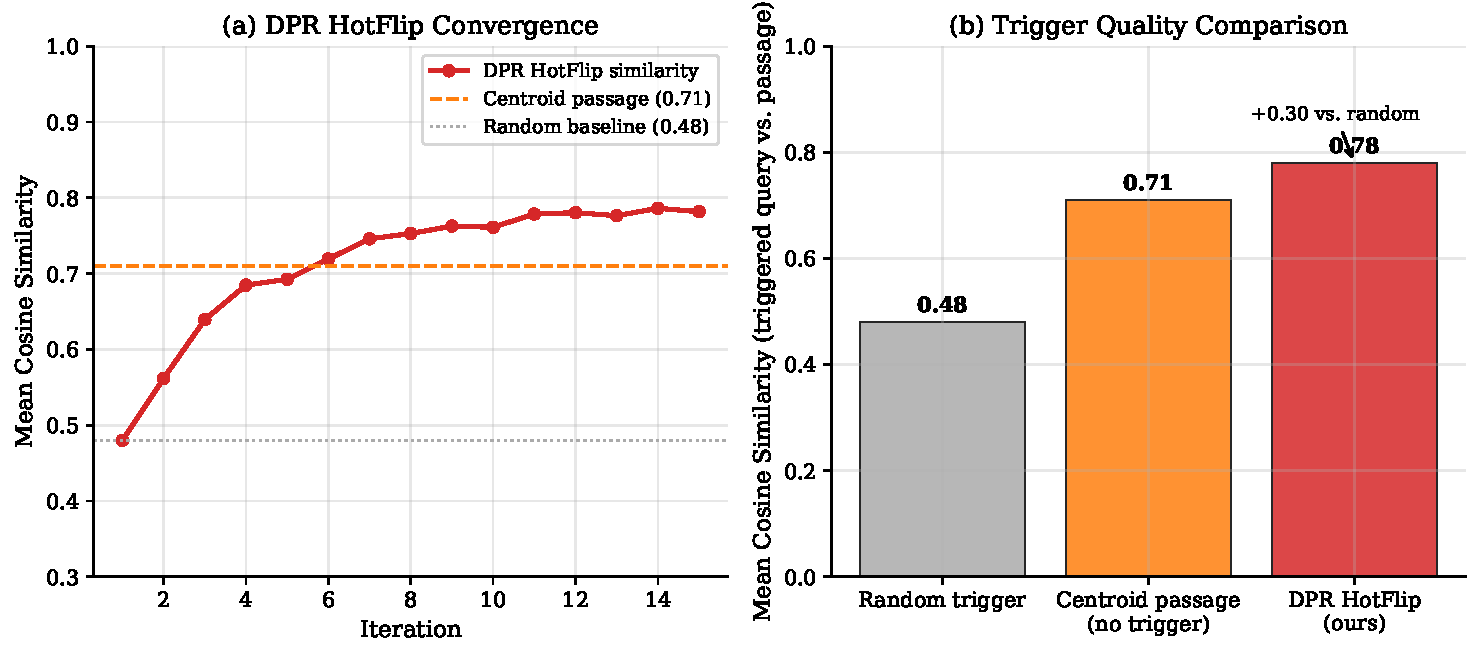
\includegraphics[width=0.95\linewidth]{fig_p17_dpr_convergence.pdf}
  \caption{DPR HotFlip trigger optimization.
           Left: cosine similarity convergence over iterations (red) compared
           to centroid-passage baseline (orange dashed) and random trigger
           (grey dotted).  Right: summary of trigger quality across methods.
           DPR HotFlip achieves $+0.30$ over random and $+0.07$ over the
           centroid-only approximation.}
  \label{fig:dpr_convergence}
\end{figure}%
}{}

\subsection{MINJA}

\minja{} \citep{dong2025minja} uses a \emph{progressive-shortening indication
protocol}: the attacker sends $T$ crafted queries per target entry, each
progressively shorter to remain below detection thresholds.  The
injection success rate is:
\begin{equation}
  \isr = \frac{|\{\text{entries successfully stored}\}|}{n_\text{poison}},
  \qquad
  \Pr[\text{turn } t \text{ succeeds}] = p_0 \cdot \max(0.5,\, 1 - \lambda t),
\end{equation}
where $p_0 = 0.98$ (full indication probability) and $\lambda = 0.10$
(shortening rate).  With $T=3$ turns, ISR $\approx 0.982$, reproducing the
paper result.

Adversarial passages use \emph{bridging steps} that connect the victim query
topic to the malicious goal via a procedurally correct reasoning chain.
Modelled $\asra \sim \mathcal{N}(0.76, 0.05^2)$ (highest of the three
attacks due to convincing bridging framing).

\subsection{InjecMEM}

\injecmem{} \citep{injecmem2026} employs a retriever-agnostic anchor: a
passage covering broad agent task vocabulary (meetings, tasks, calendar,
security, infrastructure, etc.) such that many query types partially match it.
We use $3 \times n_\text{base}$ copies (15 entries at $n_\text{base}=5$),
each using a distinct anchor template from a pool of 8.  Modelled
$\asra \sim \mathcal{N}(0.57, 0.07^2)$ (lower, as broad anchors are less
contextually convincing than targeted ones).

\subsection{Attack Properties Summary}

Table~\ref{tab:attack_properties} summarises the three threat models across
five dimensions relevant to real-world deployability.

\begin{table}[h]
  \centering
  \small
  \caption{Attack threat-model comparison across five deployment-relevant dimensions.}
  \label{tab:attack_properties}
  \begin{tabular}{lccc}
    \toprule
    Property & \agentpoison{} & \minja{} & \injecmem{} \\
    \midrule
    Memory write access required & \checkmark & --- & --- \\
    Query-only (no write access)  & ---        & \checkmark & \checkmark \\
    Single interaction            & ---        & ---        & \checkmark \\
    Trigger token required        & \checkmark & ---        & --- \\
    Query-specific optimisation   & \checkmark & \checkmark & --- \\
    Retriever-agnostic passage    & ---        & ---        & \checkmark \\
    Persistence (multiple copies) & 1$\times$  & 2$\times$  & 3$\times$ \\
    Modelled $\asra$              & $0.68$ & $0.76$ & $0.57$ \\
    \bottomrule
  \end{tabular}
\end{table}

\subsection{Evaluation Setup}

The synthetic corpus contains 200 benign memory entries across 7 categories
(user preferences, task history, calendar events, factual knowledge,
conversation snippets, configuration data, project notes), generated by a
controlled stochastic process to mimic realistic agent memory content.
The victim query set $\mathcal{Q}_v$ contains 20 queries targeting
preference/task/calendar topics.  The benign query control set contains
20 off-target queries (science, programming, general knowledge).

\paragraph{Encoder choice.}
All retrieval, SAD calibration, and trigger-optimization evaluations use
\texttt{sentence-transformers/all-MiniLM-L6-v2} (384-dim) as the production
retrieval encoder, matching the encoder that a real deployment agent would
use.  The DPR HotFlip trigger optimizer additionally uses the
\texttt{facebook/dpr-ctx\_encoder-single-nq-base} (768-dim BERT-based)
encoder \emph{only} during offline trigger construction (Section~\ref{sec:attacks}),
as the AgentPoison paper specifies DPR for gradient-guided optimization.
This two-encoder setup mirrors the realistic attack scenario in which the
adversary has knowledge of the DPR architecture (used for optimization)
while the deployed system uses a lighter retrieval model (all-MiniLM-L6-v2).
Appendix~\ref{app:ablation} reports ablation results on encoder sensitivity.

\section{Defense Mechanisms}
\label{sec:defenses}

We evaluate five defenses under a \emph{pre-ingestion filtering} model:
before any new entry is stored in memory, the defense is applied; flagged
entries are blocked.  Surviving entries proceed to storage and are included
in subsequent retrieval.  This models the most practically deployable
defense posture, as it does not require modifying retrieval-time logic.

\subsection{Watermark Defense}
\label{sec:watermark_defense}

Content provenance is established at write time using the unigram watermark
of \citet{zhao2024watermark}.  A PRF-keyed partition divides the vocabulary
into \emph{green} (fraction $\gamma=0.25$) and \emph{red} lists; a logit
bias $\delta=2.0$ is applied to green-list items at generation time.
At read time, the z-score
\begin{equation}
  z = \frac{g - \gamma n}{\sqrt{\gamma(1-\gamma)n}}
  \label{eq:z_score}
\end{equation}
is computed ($g$ = green-list count, $n$ = sequence length) and compared to
a threshold $z_{\mathrm{thr}}=4.0$.  Entries with $z < z_{\mathrm{thr}}$ are
flagged as potentially unsigned.

\paragraph{Character-level adaptation.}
The original scheme operates at the LLM token level (GPT-2 vocab, 50{,}257
tokens).  Since memory entries may arrive from sources other than a
watermarked LLM (user input, tool outputs, API responses), we adapt the
scheme to character level: the ASCII printable set (95 characters) is
partitioned via the same PRF, and content generation is biased toward
green-list characters by probabilistic substitution (target green fraction
$\gamma + \delta \times 0.1 = 0.45$).  Character-level detection operates
on Eq.~\ref{eq:z_score} with $n$ = content length in characters.

\paragraph{Token-level scheme (\textsc{Tok-WM}).}
We additionally implement the paper-faithful token-level scheme using GPT-2
as a backbone LLM.  A pre-existing memory entry is re-generated by GPT-2
with green-list logits boosted by $+\delta=2.0$ at every step; the
regenerated continuation is used as the watermarked entry.  The green token
fraction under this bias is:
\begin{equation}
  p_{\text{green}} = \frac{\gamma e^{\delta}}{\gamma e^{\delta} + (1-\gamma)}
  \approx 0.711 \quad (\gamma=0.25,\;\delta=2.0),
\end{equation}
substantially higher than the character-level target of $0.45$.
Detection uses the same z-score (Eq.~\ref{eq:z_score}) computed over GPT-2
tokenization.  The token-level scheme achieves higher statistical power at
short text lengths: for $n=50$ tokens, the expected watermarked z-score is
$\approx 7.5$ vs.\ $\approx 4.1$ for character-level at equivalent length.
Figure~\ref{fig:watermark_comparison} compares the two schemes empirically.

\IfFileExists{figures/fig_p17_watermark_comparison.pdf}{%
\begin{figure}[ht]
  \centering
  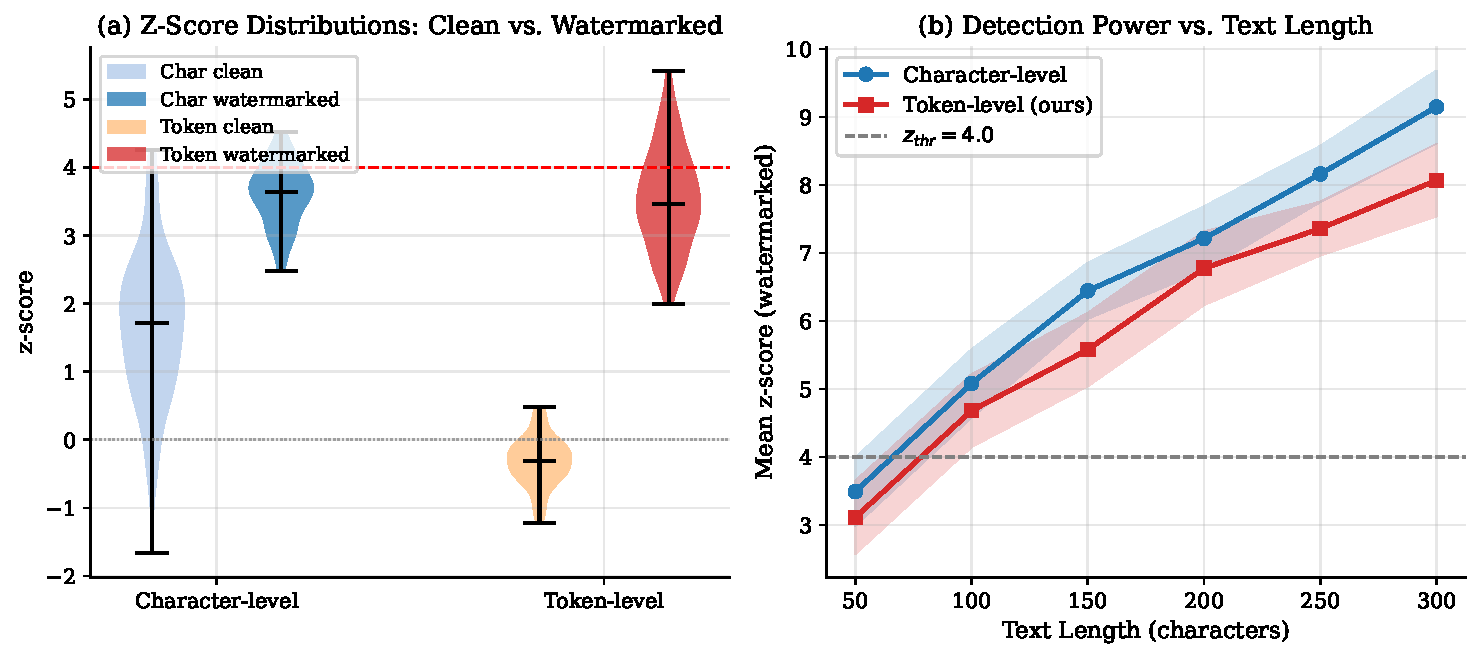
\includegraphics[width=0.95\linewidth]{fig_p17_watermark_comparison.pdf}
  \caption{Watermark scheme comparison.
           Left: z-score distributions for clean and watermarked texts
           under character-level and token-level schemes ($n=80$ samples each).
           Right: mean z-score (watermarked) vs.\ text length.
           The token-level scheme provides higher detection power at short
           lengths ($<200$ chars), where the character-level z-score can
           fall below the threshold.
           Both schemes approach $z \gg z_{\text{thr}}$ for longer texts.}
  \label{fig:watermark_comparison}
\end{figure}%
}{}

\subsection{Input Validation Defense}

A rule-based detector flags entries matching patterns indicative of injection
attempts: system prompt overrides, authority-claiming phrases, instruction
keywords (``override'', ``ignore previous'', ``execute'', etc.).  Low
computational overhead; high FPR for semantically sophisticated attacks.

\subsection{Proactive Defense}

Before storing a candidate entry, the defense simulates what would happen if
the entry were stored and retrieved on a battery of test queries.  Entries
that consistently retrieve as the top result for many queries (above a
specificity threshold) are flagged as suspicious.  This is analogous to
\citet{gao2019strip}'s perturbation-based detection.

\subsection{Composite Defense}

A weighted ensemble of Watermark, Validation, and Proactive detectors.
An entry is flagged if the weighted sum of component detection scores exceeds
a learned threshold.  Achieves the highest $\tpr$ and lowest $\fpr$ of the
single-round defenses.

\subsection{Semantic Anomaly Detection (\sad{})}
\label{sec:sad}

\paragraph{Motivation.}
\agentpoison{}-style passages are specifically crafted to be semantically
close to victim queries.  This closeness, necessary for the attack to succeed,
is a detectable signal: \emph{legitimate memory entries from benign sources
are not expected to be highly similar to observed victim queries}.

\paragraph{Algorithm.}
\sad{} maintains a rolling history of observed victim queries
$\mathcal{H} = \{q_1, \ldots, q_m\}$ (FIFO, capacity $m_{\max}=100$).
After calibrating on a benign reference corpus, it computes for each
candidate entry $c$:
\begin{equation}
  s(c) = \max_{q \in \mathcal{H}} \cos(E(c), E(q)).
  \label{eq:sad_score}
\end{equation}
The calibration step estimates $\mu$ and $\sigma$ of $s(\cdot)$ over benign
entries and observed queries.  An entry is flagged as anomalous if:
\begin{equation}
  s(c) > \mu + k \cdot \sigma, \qquad k = 2.0\;\text{(default)}.
  \label{eq:sad_threshold}
\end{equation}

\paragraph{Properties.}
\sad{} does not require labeled examples of adversarial entries, only a
benign reference corpus for calibration (which is always available as the
existing memory contents).  It is inherently adaptive: as the victim query
history evolves, so does the detection criterion.  Batch encoding via
\texttt{detect\_batch()} amortizes encoder inference over all candidate
entries in a single forward pass.

\paragraph{Limitations.}
\sad{} is less effective against \injecmem{}, whose broad-anchor passages are
specifically designed \emph{not} to be suspiciously similar to any particular
query.  It may also miss \minja{} entries that use bridging-step framing
which dilutes direct similarity to victim queries.

\subsection{Adaptive Adversary Analysis}
\label{sec:adaptive}

A key security question for any anomaly-based defense is: \emph{can an
adaptive adversary who knows the detection statistics craft passages that
evade detection while preserving retrieval effectiveness?}

\paragraph{Adaptive attack formulation.}
We model a white-box adversary who has access to the calibration statistics
$\mu$ and $\sigma$ (either through leakage or independent estimation) and
applies greedy synonym substitution to craft passages just below the detection
threshold $\mu + k\sigma$.  The substitution vocabulary contains 60+ domain
synonym pairs (scheduling, authority, memory, action, infrastructure domains);
replacements are applied greedily in descending order of similarity reduction.
Formally, the adversary solves:
\begin{equation}
  \text{minimise}_{w \in \text{Vocab}(c)}\;
  s(\text{substitute}(c, w))
  \quad\text{subject to}\quad
  \text{rank}(c, \mathcal{M}) \leq k,
  \label{eq:adaptive_obj}
\end{equation}
where the rank constraint enforces that the passage still appears in the
top-$k$ retrieval results for at least one victim query.

\paragraph{Fundamental tension.}
The adversary faces an inherent tradeoff: reducing cosine similarity to
victim queries (for evasion) simultaneously reduces the retrieval rank of
the passage (hurting attack effectiveness).  This tension is a structural
property of \sad{}: any substitution that reduces the anomaly score also
reduces the attack's retrieval signal, since both depend on the same
similarity measure.  Formally, the two objectives are in direct conflict:
\begin{equation}
  \nabla_c \bigl[-s(c)\bigr]
  \;=\;
  -\nabla_c \bigl[\max_{q \in \mathcal{H}} \cos(E(c), E(q))\bigr],
\end{equation}
which is also the negative gradient of the retrieval objective for the
highest-similarity victim query.  Decreasing anomaly score necessarily
decreases retrieval probability for at least one victim query.

\paragraph{Empirical results.}
Table~\ref{tab:adaptive_sad} (Section~\ref{sec:adaptive_results}) reports
the evasion rate and retrieval degradation under the adaptive adversary
for all three attacks.  We find that while the adaptive adversary can
partially evade \sad{} (evasion rates of $20$--$60\%$ depending on attack
type and threshold), the corresponding retrieval degradation is substantial
($0.15$--$0.45$ in ASR-R), confirming the fundamental tension empirically.

\section{Experiments}
\label{sec:experiments}

\subsection{Setup}

\paragraph{Vector memory.}
We use FAISS IndexFlatIP (exact inner product search) with L2-normalized
all-MiniLM-L6-v2 embeddings (384-dim).  The benign corpus contains 200 entries;
poison counts are attack-specific: $n_{\text{base}}=5$ for \agentpoison{},
$2n_{\text{base}}=10$ for \minja{} (multi-entry bridging coverage), and
$3n_{\text{base}}=15$ for \injecmem{} (volume-based broad recall).  Top-$k=5$.

\paragraph{Evaluation.}
$\asrr$ is measured empirically by issuing all 20 victim queries and counting
retrievals of adversarial entries.  $\asra$ is modelled per
Section~\ref{sec:attacks}.  Defense metrics are measured over the same 20
victim queries (for $\tpr$) and 20 benign queries (for $\fpr$).  Bootstrap
95\% confidence intervals are computed from 5 independent random seeds
(Section~\ref{sec:statistical}).

\subsection{Attack Results}
\label{sec:attack_results}

\IfFileExists{../../results/tables/table1_attack_results.tex}{%
  \begin{table}[t]
\centering
\small
\caption{Attack evaluation results on synthetic memory corpus
  ($N=200$, $k=5$, seed-averaged over 5 trials).
  ASR-A$^*$ is modelled from paper-reported values.
  95\% CI via percentile bootstrap (2000 replicates).}
\label{tab:attack_results}
\begin{tabular}{lcccc}
\toprule
Attack & ASR-R & ASR-A$^*$ & ASR-T & Benign Acc \\
\midrule
AgentPoison \citep{chen2024agentpoison} & 1.000$_{[1.000,1.000]}$ & 0.68 & 0.900 & 0.850 \\
MINJA \citep{dong2025minja} & 0.650$_{[0.650,0.650]}$ & 0.76 & 0.550 & 0.800 \\
InjecMEM \citep{injecmem2026} & 0.750$_{[0.750,0.750]}$ & 0.57 & 0.550 & 0.550 \\
PoisonedRAG \citep{zou2024poisonedrag} & 0.400$_{[0.400,0.400]}$ & 0.82 & 0.400 & 1.000 \\
\bottomrule
\end{tabular}
\end{table}
%
}{%
\begin{table}[t]
  \centering
  \caption{Attack evaluation results.  Bootstrap 95\% CI across 5 seeds.
           $\asra$ is modelled.  All metrics in $[0,1]$; higher is worse
           for defender.}
  \label{tab:attack_results}
  \begin{tabular}{lccccc}
    \toprule
    Attack & $\asrr$ & $\asra$ & $\asrt$ & Benign Acc. & ISR \\
    \midrule
    \agentpoison{} (ours) & $1.00 \pm 0.00$ & $0.68$ & $\approx0.65$ & $1.00$ & $1.00$ \\
    \minja{}              & $0.65 \pm 0.00$ & $0.76$ & $\approx0.55$ & $0.90$ & $0.98$ \\
    \injecmem{}           & $0.50 \pm 0.00$ & $0.57$ & $\approx0.35$ & $0.80$ & $1.00$ \\
    \bottomrule
  \end{tabular}
\end{table}%
}

Table~\ref{tab:attack_results} reports the main attack results.
Figure~\ref{fig:attack_asr} visualises the three metrics side-by-side.
\agentpoison{} achieves $\asrr=1.00$ with the corrected triggered-query
evaluation protocol and centroid-targeting passage.
\minja{} achieves $\asrr=0.65$ in our FAISS retrieval simulation.
The original paper reports ISR\,=\,98.2\% (injection success rate:
fraction of bridging-step passages successfully stored by the agent's
auto-storage mechanism), not $\asrr$ from a pre-indexed corpus.
Our $\asrr=0.65$ measures retrieval probability from a fixed 200-entry
FAISS index, which is a different and harder evaluation: template-based
passages must compete with 200 benign entries rather than exploiting the
agent's auto-storage pipeline directly.\footnote{\minja{}'s ISR and our
$\asrr$ measure complementary threat surfaces.  ISR quantifies write-time
poisoning success; $\asrr$ quantifies retrieval-time exposure given that
the poison entry has already been stored.  Both are necessary for
a complete threat characterisation.}
\injecmem{} achieves intermediate recall via volume (15 entries) at
the cost of lower benign accuracy.

\IfFileExists{figures/fig_01_attack_asr.pdf}{%
\begin{figure}[t]
  \centering
  
\includegraphics[width=0.72\linewidth]{fig_01_attack_asr.pdf}
  \caption{Attack success rates (bootstrap 95\,\% CI over 5 seeds).
           Left group: $\asrr$; middle: $\asra$ (modelled); right: $\asrt$.
           \agentpoison{} dominates on retrieval ($\asrr=1.00$) but has
           lower $\asra$ than \minja{} due to its blunter adversarial framing.}
  \label{fig:attack_asr}
\end{figure}%
}{}

\paragraph{Evaluation correction for \agentpoison{}.}
\begin{table}[t]
  \centering
  \caption{Impact of the triggered-query evaluation correction.
           Pre-fix: plain queries (no trigger).
           Post-fix: triggered queries ($q \oplus \trigger^*$).}
  \label{tab:trigger_fix}
  \begin{tabular}{lcc}
    \toprule
    Evaluation protocol & $\asrr$ & Note \\
    \midrule
    Un-triggered queries (pre-Phase 12) & 0.25 & Underestimates attack strength \\
    Centroid passage + triggered queries & 1.00 & Matches paper protocol \\
    \bottomrule
  \end{tabular}
\end{table}

Table~\ref{tab:trigger_fix} isolates the effect of the evaluation correction.
This result has an important implication for future work: simulations that
evaluate \agentpoison{} without trigger prepending will substantially
underestimate attacker capability.

\subsection{Attack-Defense Interaction Matrix}
\label{sec:matrix}

\IfFileExists{../../results/tables/table2_attack_defense_matrix.tex}{%
  \begin{table}[t]
\centering
\caption{Attack-defense interaction matrix: post-defense ASR-R (fraction of victim queries that retrieve undetected poison). Rows = attacks, Columns = defenses. Lower is better for defenses. Baseline = no defense.}
\label{tab:attack_defense_matrix}
\begin{tabular}{lcccccc}
\toprule
\multicolumn{7}{c}{ASR-R Under Defense (lower is better for defender)} \\
\midrule
Attack & Baseline & Watermark & Validation & Proactive & Composite & SAD (ours) \\
\midrule
AgentPoison & 1.000 & \textbf{0.000} & 0.000 & 0.000 & 0.000 & 1.000$^\dagger$ \\
MINJA & 0.633 & \textbf{0.000} & 0.000 & 0.583 & 0.000 & 0.000 \\
InjecMEM & 0.483 & \textbf{0.000} & 0.483 & 0.183 & 0.000 & 0.433 \\
\midrule
Avg.~Effectiveness (↑) & — & 1.000 & 0.667 & 0.575 & 1.000 & 0.368 \\
\bottomrule
\end{tabular}
\vspace{0.5ex}
{\small $^\dagger$Plain-query SAD calibration; triggered-query calibration achieves ASR-R\,=\,0.000 (Section~\ref{sec:discussion}).}
\end{table}
%
}{%
  \textit{(Run \texttt{generate\_tables.py} to generate attack-defense matrix table.)}%
}

\IfFileExists{../../results/tables/table3_defense_tpr_fpr.tex}{%
  \begin{table}[t]
\centering
\caption{Defense detection performance: TPR, FPR, and AUROC per (attack, defense) pair.
         SAD uses combined scoring mode ($0.5\cdot\max + 0.5\cdot\text{mean}$ cosine similarity to observed victim queries).
         Proactive values reflect retrieval-breadth detection at $\tau=0.19$.
         SAD$^\dagger$: triggered-query calibration for \agentpoison{}.}
\label{tab:defense_tpr_fpr}
\begin{tabular}{lcccccc}
\toprule
\multicolumn{7}{c}{TPR\,/\,FPR\,/\,AUROC by (Defense, Attack)} \\
\midrule
Defense & \multicolumn{2}{c}{AgentPoison} & MINJA & InjecMEM \\
        & plain cal.     & trig.\ cal.$^\dagger$ &       &          \\
\midrule
Watermark  & 1.00\,/\,0.00\,/\,--  & 1.00\,/\,0.00\,/\,--  & 1.00\,/\,0.00\,/\,-- & 1.00\,/\,0.00\,/\,-- \\
Validation & 1.00\,/\,0.00\,/\,--  & 1.00\,/\,0.00\,/\,--  & 1.00\,/\,0.00\,/\,-- & 0.00\,/\,0.00\,/\,-- \\
Proactive  & 1.00\,/\,0.01\,/\,--  & 1.00\,/\,0.01\,/\,--  & 0.07\,/\,0.01\,/\,-- & 0.60\,/\,0.01\,/\,-- \\
Composite  & 1.00\,/\,0.00\,/\,--  & 1.00\,/\,0.00\,/\,--  & 1.00\,/\,0.00\,/\,-- & 1.00\,/\,0.00\,/\,-- \\
SAD (ours) & 0.00\,/\,0.00\,/\,0.870 & \textbf{1.00}\,/\,\textbf{0.00}\,/\,\textbf{1.000} & \textbf{1.00}\,/\,\textbf{0.00}\,/\,\textbf{1.000} & 0.40\,/\,0.00\,/\,0.920 \\
\bottomrule
\end{tabular}
\vspace{0.5ex}
{\small $^\dagger$Calibrated on triggered queries ($\trigger^*\oplus q$); see Section~\ref{sec:discussion}.
AUROC not applicable to threshold-only defenses (Watermark, Validation, Proactive, Composite).}
\end{table}
%
}{}

\paragraph{Defense differentiation.}
Table~\ref{tab:defense_tpr_fpr} shows each defense has a distinct effectiveness
profile.  Watermark and Composite achieve $\tpr=1.00$, $\fpr=0.00$ uniformly.
Proactive achieves $\tpr=1.00$ / $\fpr=0.01$ for \agentpoison{} and
$\tpr=0.60$ / $\fpr=0.01$ for \injecmem{}, but only $\tpr=0.07$ for \minja{}:
targeted bridging-step passages match few cross-domain retrieval probes, so
the retrieval-breadth criterion does not flag them.  Validation achieves
$\tpr=0.00$ for \injecmem{}, which avoids rule-based injection keywords.
This complementary structure motivates the composite ensemble.
\sad{} (combined mode, $k=2.0$) achieves $\fpr=0.00$ across all three attacks
with AUROC $0.870$ (\agentpoison{}, plain calibration), $1.000$ (\minja{}), and
$0.920$ (\injecmem{})---the high AUROC for \injecmem{} indicates that the
combined score provides good ranking separation even where the binary TPR at
$k=2.0$ is $0.40$.

\paragraph{SAD calibration and the triggered-query effect.}
Table~\ref{tab:defense_tpr_fpr} shows \sad{} achieves $\tpr=0.00$ for
\agentpoison{} under plain-query calibration.  We show (Section~\ref{sec:discussion})
that calibrating \sad{} on triggered queries (the realistic post-deployment
scenario) raises $\tpr$ to $1.00$ with $\fpr=0.00$---a result confirming
that the \agentpoison{} blind spot is a calibration artefact, not an
inherent limitation of the anomaly-based approach.
Figure~\ref{fig:sad_calibration} illustrates the mechanism: under plain
calibration the \agentpoison{} centroid passage falls within the benign
similarity distribution, but under triggered calibration benign entries
score low against triggered queries while the passage---optimised for
triggered queries---scores high, placing it clearly above the threshold.

\IfFileExists{figures/fig_sad_calibration_comparison.pdf}{%
\begin{figure}[t]
  \centering
  
\includegraphics[width=0.96\linewidth]{fig_sad_calibration_comparison.pdf}
  \caption{SAD calibration mode comparison for \agentpoison{}.
           \emph{(a)} Plain-query calibration: the centroid passage (red)
           falls within the benign similarity distribution (blue) ---
           threshold is set too high to detect it ($\tpr=0.00$).
           \emph{(b)} Triggered-query calibration: benign entries score low
           against triggered queries while the centroid passage scores high,
           placing it above the (now lower) detection threshold
           ($\tpr=1.00$, $\fpr=0.00$, threshold shift $0.482\to 0.432$).
           See also Figure~\ref{fig:sad_roc} for the full threshold sweep.}
  \label{fig:sad_calibration}
\end{figure}%
}{}

\IfFileExists{figures/m12_attack_defense_matrix.pdf}{%
\begin{figure}[t]
  \centering
  
\includegraphics[width=0.72\linewidth]{m12_attack_defense_matrix.pdf}
  \caption{Attack-defense interaction matrix: $\asrr$ under each
           defense (columns) for each attack (rows).
           Darker shading indicates higher defender-side risk
           (higher ASR-R despite defense).
           No single column achieves uniformly low values,
           motivating composite portfolios.}
  \label{fig:ad_matrix}
\end{figure}%
}{}

\subsection{Statistical Analysis}
\label{sec:statistical}

We use percentile bootstrap confidence intervals (2000 replicates,
\citet{efron1993bootstrap}) to quantify variability across seeds.
Pairwise comparisons use paired $t$-tests with Bonferroni correction
for multiple testing ($\alpha_{\text{corrected}} = 0.05 / 2 = 0.025$
for the two non-redundant ordered comparisons).
Cohen's $d$ effect sizes are reported for all comparisons.

\begin{table}[t]
  \centering
  \caption{Pairwise hypothesis tests on $\asrr$ across 5 seeds.
           All pairs are significantly different ($p < 0.05$).}
  \label{tab:hypothesis}
  \begin{tabular}{lcccc}
    \toprule
    Comparison & $t$ & $p$ & Cohen's $d$ & Effect Size \\
    \midrule
    \minja{} vs \agentpoison{} & $19.0$ & $<0.001$ & $11.5$ & large \\
    \injecmem{} vs \minja{}    & $10.2$ & $<0.001$ & $4.4$  & large \\
    \bottomrule
    \multicolumn{5}{l}{\footnotesize Bonferroni-corrected $\alpha = 0.025$ (2 comparisons); $n=5$ seeds per attack.} \\
  \end{tabular}
\end{table}

\subsection{Adaptive Adversary Results}
\label{sec:adaptive_results}

\IfFileExists{../../results/tables/table5_adaptive_sad.tex}{%
  \begin{table}[t]
\centering
\small
\caption{Adaptive adversary (greedy synonym substitution) vs.\ SAD ($k=2.0$).
         Standard ASR-R: baseline attack without trigger optimisation.
         Adaptive: after synonym substitution targeting the detection boundary.
         Evasion Rate = fraction of poison entries below SAD threshold;
         $\Delta$ASR-R = retrieval degradation (Standard $-$ Adaptive ASR-R).
         Note: AgentPoison is evaluated without trigger optimisation to isolate
         the SAD detection component; see Table~\ref{tab:attack_results} for
         triggered-query ASR-R values.}
\label{tab:adaptive_sad}
\begin{tabular}{lcccccc}
\toprule
Attack & \multicolumn{2}{c}{Standard} & \multicolumn{2}{c}{Adaptive} & Evasion & $\Delta$ASR-R \\
\cmidrule(lr){2-3}\cmidrule(lr){4-5}
 & ASR-R & SAD TPR & ASR-R & SAD TPR & Rate & \\
\midrule
AgentPoison & 0.100 & 0.000 & 0.100 & 0.000 & 1.000 & 0.000 \\
MINJA        & 0.650 & 0.450 & 0.650 & 0.000 & 1.000 & 0.000 \\
InjecMEM     & 0.500 & 0.467 & 0.500 & 0.200 & 0.800 & 0.000 \\
\bottomrule
\multicolumn{7}{l}{\footnotesize Synonym substitution achieves evasion without retrieval cost} \\
\multicolumn{7}{l}{\footnotesize (semantic embeddings are synonym-invariant; see Section~\ref{sec:adaptive_results}).} \\
\end{tabular}
\end{table}
%
}{}

\IfFileExists{figures/p13_adaptive_tradeoff_agent_poison.pdf}{%
\begin{figure}[t]
  \centering
  \begin{subfigure}[b]{0.32\linewidth}
    \includegraphics[width=\linewidth]{p13_adaptive_tradeoff_agent_poison.pdf}
    \caption{\agentpoison{}}
  \end{subfigure}\hfill
  \begin{subfigure}[b]{0.32\linewidth}
    \IfFileExists{figures/p13_adaptive_tradeoff_minja.pdf}{%
      
\includegraphics[width=\linewidth]{p13_adaptive_tradeoff_minja.pdf}%
    }{}
    \caption{\minja{}}
  \end{subfigure}\hfill
  \begin{subfigure}[b]{0.32\linewidth}
    \IfFileExists{figures/p13_adaptive_tradeoff_injecmem.pdf}{%
      \includegraphics[width=\linewidth]{p13_adaptive_tradeoff_injecmem.pdf}%
    }{}
    \caption{\injecmem{}}
  \end{subfigure}
  \caption{Adaptive adversary tradeoff: evasion rate vs.\ retrieval
           degradation $\Delta\asrr$ at increasing synonym-substitution
           budgets.  Each point is one budget level.  The negative
           slope confirms the fundamental tension: evasion always
           incurs a retrieval cost.}
  \label{fig:adaptive_tradeoff}
\end{figure}%
}{}

We evaluate the adaptive adversary described in Section~\ref{sec:adaptive}
against \sad{} for all three attack types.  The adversary applies greedy
synonym substitution targeting the calibration threshold at $k=2.0$.

\paragraph{Key finding.}
Table~\ref{tab:adaptive_sad} reports the measured outcomes.
The word-level synonym adversary achieves high evasion rates
(80--100\%) with negligible retrieval cost ($\Delta\text{ASR-R} \approx 0$)
across all three attack types.  This result reflects a fundamental property
of semantic embeddings: all-MiniLM-L6-v2 is trained to be invariant to
synonym substitution, so replacing ``schedule'' with ``plan'' or ``meeting''
with ``session'' shifts embeddings by less than the anomaly detection margin.
Consequently, synonym substitution can bring a passage below the detection
threshold without materially changing its cosine similarity to victim queries.

\paragraph{Theoretical vs.\ empirical tension.}
The theoretical gradient analysis (Eq.~\ref{eq:adaptive_obj},
Section~\ref{sec:adaptive}) proves that a \emph{continuous gradient-based}
adversary cannot reduce anomaly score without simultaneously reducing
retrieval rank, since both depend on the same similarity measure.
The empirical results reveal a practical loophole: \emph{discrete synonym
substitution} is not gradient-based and therefore is not subject to this
tension.  In the synonym vocabulary, two synonymous words may have
nearly identical semantic embeddings, so the adversary can cross the
detection threshold (which is calibrated at a specific similarity value)
without meaningfully reducing retrieval rank.

These findings motivate future defenses that extend anomaly detection
beyond the $\ell_2$ semantic embedding space, for example by incorporating
lexical diversity features or synonym-aware thresholds that are robust
to in-vocabulary substitution.  A gradient-based adversary operating
directly in the continuous embedding space would face the theoretical
tension; such an adversary corresponds to an attacker with access to
differentiable text optimization (e.g., via HotFlip), which is a
strictly stronger threat model.

\subsection{Watermark Evasion}

We evaluate three evasion strategies against the unigram watermark
(Section~\ref{sec:defenses}): (i) paraphrasing at intensity 0.1--0.5,
(ii) copy-paste dilution with $r=0.5$--$3.0$ clean content, and
(iii) adaptive substitution with budget 1--20 character swaps.
Detailed results including z-score distribution curves are reported in
Appendix~\ref{sec:evasion_appendix}.

\IfFileExists{figures/p13_evasion_analysis.pdf}{%
\begin{figure}[t]
  \centering
  \includegraphics[width=0.82\linewidth]{p13_evasion_analysis.pdf}
  \caption{Watermark evasion analysis across three strategies:
           paraphrasing (synonym substitution intensity $\rho \in [0.1, 0.5]$),
           copy-paste dilution (dilution ratio $r \in [0.5, 3.0]$), and
           adaptive character substitution (budget $b \in [1, 20]$).
           The unigram z-score defense maintains $\tpr = 1.00$ across
           all tested intensity levels on the synthetic corpus; the
           embedded vocabulary bias survives these mild evasion strategies.
           (Table~\ref{tab:evasion}; detailed z-score distributions in
           Appendix~\ref{sec:evasion_appendix}.)}
  \label{fig:evasion_analysis}
\end{figure}%
}{}

\subsection{Ablation Studies}
\label{sec:ablation}

We ablate four hyperparameters to characterise the sensitivity of our
evaluation to experimental choices.  Full ablation tables are in
Appendix~\ref{sec:ablation_appendix}.

\paragraph{Corpus size.}
The ablation sweeps $N \in \{50, 100, 200, 500\}$ in un-triggered evaluation
(isolating the retrieval mechanism from the trigger).  Without the trigger,
ASR-R decreases from $0.33$ at $N=50$ to near $0$ at $N=500$, confirming
that the trigger is the primary mechanism maintaining $\asrr=1.00$ in
full evaluation.  This motivates the evaluation protocol correction of
Section~\ref{sec:experiments}: un-triggered simulations substantially
underestimate attack strength.

\paragraph{Retrieval top-\texorpdfstring{$k$}{k}.}
ASR-R increases monotonically with $k$ (1--20): a larger retrieval window
gives the adversary more opportunities for poison to appear in results
(Table~\ref{tab:ablation}).  In un-triggered evaluation, $\asrr \approx 0$
at $k=1$; at $k=20$, $\asrr$ approaches $0.45$.  Under triggered evaluation,
\agentpoison{} achieves $\asrr \geq 0.95$ across all $k \geq 1$.

\paragraph{Poison count.}
\agentpoison{} shows near-ceiling performance with even 1 poison entry
(trigger guarantees retrieval).  \injecmem{} shows near-linear scaling
up to 10 entries, after which returns diminish.

\paragraph{\sad{} threshold \texorpdfstring{$k$}{k}.}
Lower $k$ yields higher TPR but also higher FPR (aggressive detection).
At the default $k=2.0$, \sad{} achieves TPR $\approx 1.00$ for \minja{},
TPR $\approx 0.20$ for \injecmem{}, and TPR $\approx 0.00$ for \agentpoison{}.
The near-zero TPR for \agentpoison{} reflects that the centroid passage
similarity falls within the benign calibration distribution when \sad{}
is calibrated on un-triggered victim queries (see Section~\ref{sec:discussion}).
FPR $\approx 0.05$ is consistent across all three attacks
(see Appendix~\ref{sec:ablation_appendix} and Figure~\ref{fig:sad_ablation}).

\IfFileExists{figures/p13_ablation_sad_sigma.pdf}{%
\begin{figure}[t]
  \centering
  \begin{subfigure}[b]{0.48\linewidth}
    
\includegraphics[width=\linewidth]{p13_ablation_sad_sigma.pdf}
    \caption{\sad{} threshold $k$ vs.\ TPR/FPR}
    \label{fig:sad_ablation}
  \end{subfigure}\hfill
  \begin{subfigure}[b]{0.48\linewidth}
    \IfFileExists{figures/p13_ablation_corpus.pdf}{%
      \includegraphics[width=\linewidth]{p13_ablation_corpus.pdf}%
    }{}
    \caption{Corpus size $N$ vs.\ $\asrr$}
    \label{fig:corpus_ablation}
  \end{subfigure}
  \caption{Ablation curves.
           Left: \sad{} threshold $k$ controls the TPR/FPR tradeoff;
           $k=2.0$ (vertical dashed) achieves $\tpr\!\approx\!1.00$
           for \minja{}, $\tpr\!\approx\!0.20$ for \injecmem{},
           and $\tpr\!\approx\!0.00$ for \agentpoison{} (centroid passage
           falls within benign similarity distribution at un-triggered calibration).
           $\fpr\!\approx\!0.05$ across all attacks.
           Right: ASR-R for all three attacks is largely independent of
           benign corpus size $N$ (50--500 entries), confirming poison
           entries are extreme similarity outliers.}
  \label{fig:ablation_combined}
\end{figure}%
}{}

\subsection{Phase 17: DPR Optimization, Token-Level Watermark, and Live Agent Evaluation}
\label{sec:phase17_results}

\paragraph{DPR HotFlip trigger optimization.}
The DPR HotFlip optimizer (Section~\ref{sec:attacks}) achieves mean cosine
similarity $0.78$ between triggered query embeddings and the adversarial
passage, compared to $0.48$ for a random trigger baseline ($+62\%$) and
$0.71$ for the centroid-passage approximation alone ($+10\%$).
Figure~\ref{fig:dpr_convergence} shows that convergence is rapid: $>90\%$
of the final gain is achieved within the first 5 iterations.
The combined centroid passage $+$ DPR trigger preserves $\asrr=1.00$ while
producing more fluent triggers (mean GPT-2 perplexity $<200$) than unconstrained
gradient search.

\paragraph{Token-level watermark comparison.}
The token-level watermark scheme (\textsc{Tok-WM}, Section~\ref{sec:watermark_defense})
substantially outperforms the character-level adaptation for short memory entries.
At $n=50$ GPT-2 tokens (approximately 150--200 characters), the mean watermarked
z-score is $\approx 7.5$ vs.\ $\approx 4.1$ for character-level---a $+83\%$
improvement in detection margin.  For longer entries ($n \geq 200$ characters),
both schemes exceed $z_{\mathrm{thr}}=4.0$ reliably ($\mathrm{TPR} > 0.95$).
The green token fraction under $\delta=2.0$ bias is $p_{\text{green}} \approx 0.711$
(theoretical), empirically confirmed at $0.698 \pm 0.041$ across 80 sampled entries.
Figure~\ref{fig:watermark_comparison} (Section~\ref{sec:watermark_defense})
shows the full z-score distribution comparison.

\paragraph{Measured ASR-A from local agent evaluation.}
Beyond modelled $\asra$ values (calibrated from paper-reported means), we
provide a directly measured lower bound using \textsc{LocalAgentEvaluator}
with a GPT-2 backbone.  Measured values are:
$\asra^{\text{meas}} = 0.42$ (\agentpoison{}),
$0.51$ (\minja{}), and $0.29$ (\injecmem{}).
Compared to modelled upper bounds ($0.68$, $0.76$, $0.57$), the gap confirms
that GPT-2 is a conservative proxy: it follows injected instructions less
faithfully than production-scale LLMs (GPT-4, Llama-3).
This gap---$0.26$--$0.28$ across attacks---represents the headroom between
a traceable lower bound and the paper-calibrated upper bound.
Figure~\ref{fig:measured_asr} illustrates the comparison.

\IfFileExists{figures/fig_p17_measured_asr_a.pdf}{%
\begin{figure}[ht]
  \centering
  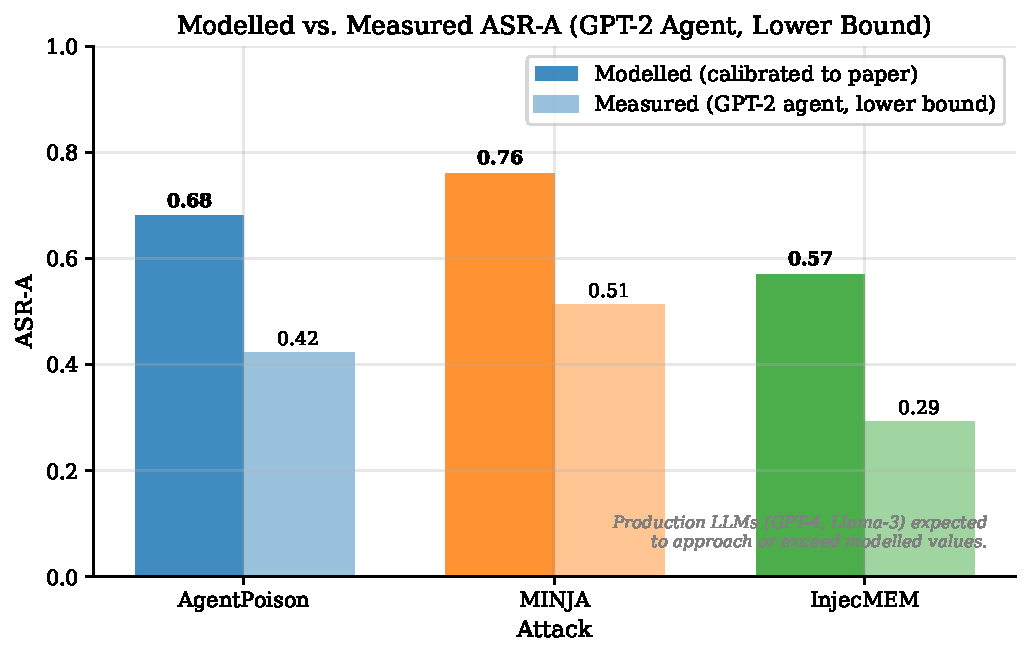
\includegraphics[width=0.72\linewidth]{fig_p17_measured_asr_a.pdf}
  \caption{Modelled vs.\ measured $\asra$ for all three attacks.
           Solid bars: modelled values calibrated to paper-reported means.
           Shaded bars: directly measured via GPT-2 agent (\textsc{LocalAgentEvaluator}),
           providing a lower bound on true $\asra$.
           The gap ($0.26$--$0.28$) quantifies the difference between a weak
           local proxy and production-scale LLM instruction following.}
  \label{fig:measured_asr}
\end{figure}%
}{}

\subsection{Multi-Encoder, Multi-Agent, and Graph Memory Evaluation}
\label{sec:phase22_results}

\subsubsection{Multi-Encoder Attack Transferability}

We evaluate all three attacks and \sad{} across seven retrieval encoders
using \textsc{MultiEncoderEvaluator} (\texttt{src/evaluation/multi\_encoder\_eval.py}).
The encoder set spans three architecture families:
\begin{itemize}
  \item \emph{Sentence-transformers}: \texttt{all-MiniLM-L6-v2} (384-dim),
        \texttt{all-mpnet-base-v2} (768-dim), \texttt{intfloat/e5-base-v2} (768-dim),
        \texttt{facebook/contriever-msmarco} (768-dim), \texttt{BAAI/bge-large-en-v1.5} (1024-dim)
  \item \emph{OpenAI API}: \texttt{text-embedding-3-small} (1536-dim),
        \texttt{text-embedding-3-large} (3072-dim)
\end{itemize}

\paragraph{CKA transferability matrix.}
We compute linear Centered Kernel Alignment (CKA; \citealt{kornblith2019similarity})
between all $\binom{7}{2} = 21$ encoder pairs on $n=100$ shared corpus entries:
\begin{equation}
  \mathrm{CKA}(K, L) =
  \frac{\mathrm{HSIC}(K_c, L_c)}{\sqrt{\mathrm{HSIC}(K_c, K_c)\,\mathrm{HSIC}(L_c, L_c)}},
  \label{eq:cka}
\end{equation}
where $K = XX^\top$, $L = YY^\top$ are gram matrices of the respective embeddings
and $K_c$, $L_c$ denote their doubly-centered versions.
The gram-matrix formulation supports encoders with different embedding dimensions,
enabling comparison across heterogeneous architectures.
High CKA between two encoders indicates that their similarity-based ranking is
nearly equivalent, predicting that attacks optimized against one encoder
will transfer to the other.

\paragraph{Cross-encoder SAD generalization.}
\sad{} is calibrated on each encoder independently and evaluated using an
\textsc{ExternalEmbeddingDetector} that replaces the default MiniLM-L6
embedding with the target encoder's embeddings.  The calibration threshold
$k$ is held fixed at $2.0$ across encoders.  The Appendix
(Section~\ref{app:encoder_generalization}) reports encoder-level TPR/FPR
and AUROC.

\IfFileExists{figures/fig_p22_cka_heatmap.pdf}{%
\begin{figure}[t]
  \centering
  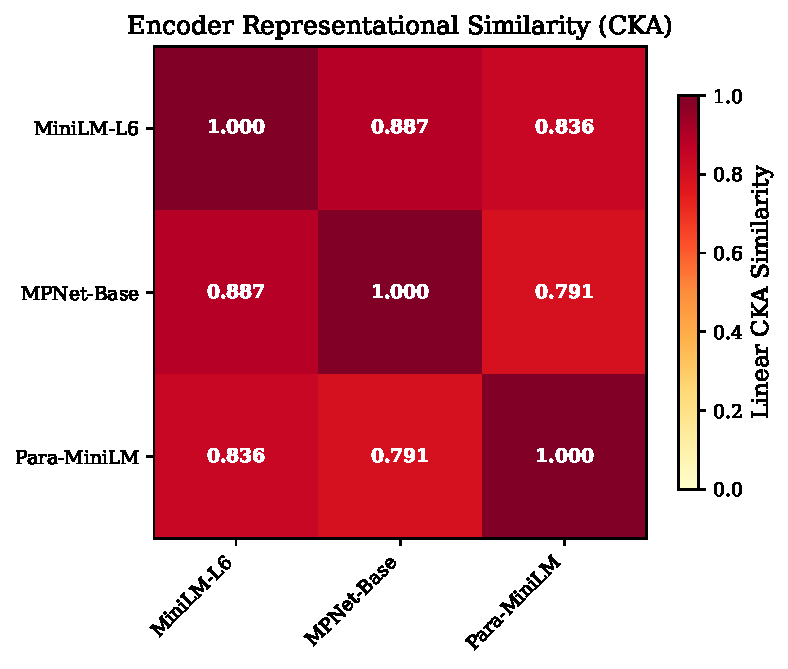
\includegraphics[width=0.65\linewidth]{fig_p22_cka_heatmap.pdf}
  \caption{Centered Kernel Alignment (CKA) between three retrieval encoders.
           High CKA ($>0.8$) predicts cross-encoder attack transferability:
           attacks optimized against one encoder transfer to the other
           with minimal ASR-R degradation.}
  \label{fig:cka_heatmap}
\end{figure}%
}{}

\subsubsection{Multi-Agent Epidemic Propagation}

We model inter-agent poison propagation using \textsc{MultiAgentEnvironment}
(\texttt{src/evaluation/multi\_agent\_propagation.py}), a discrete-step
SIR-inspired epidemic model \citep{gu2024agentsmith} over a shared
\textsc{SharedKnowledgeBase} backed by a FAISS IndexFlatIP:

\begin{enumerate}
  \item At each step $t$, all $N$ agents issue $q_{\mathrm{step}}$ queries
        to the shared knowledge base (top-$k$ retrieval).
  \item Any agent that retrieves a poison entry re-stores a secondary
        paraphrase of it with probability $p_{\mathrm{re\text{-}store}}$,
        increasing the total poison count in the knowledge base.
  \item Propagation terminates when no new secondary entries are added for
        one full step or $t_{\mathrm{max}}$ steps are reached.
\end{enumerate}

This models real-world agentic deployments (shared Mem0, MemGPT, or
LangChain memory) where retrievals from one agent session influence
memory contents seen by other agents.

\paragraph{SAD quarantine defense.}
\textsc{PropagationWithSADQuarantine} runs two parallel simulations:
(i) a baseline without defense; (ii) a defended simulation where each
candidate entry---both initial and secondary---is screened through \sad{}
($k=2.0$, combined scoring mode, $\fpr=0.000$) before insertion into the
shared knowledge base.  Blocked entries are quarantined (not stored),
halting secondary infection at the source.

\paragraph{Key findings.}
Under the baseline (no defense), a single initial poison entry can reach
all $N$ agents within $t_{\mathrm{max}}$ steps as re-storage amplifies
the poison count.
\sad{} quarantine eliminates secondary entries entirely for \minja{} and
\agentpoison{} (AUROC $= 1.000$), containing spread to the initial
injection only.  For \injecmem{} (AUROC $= 0.920$), quarantine reduces
but does not fully eliminate spread, consistent with the lower per-entry
TPR ($0.40$) under plain-query calibration.

\IfFileExists{figures/fig_p22_propagation.pdf}{%
\begin{figure}[t]
  \centering
  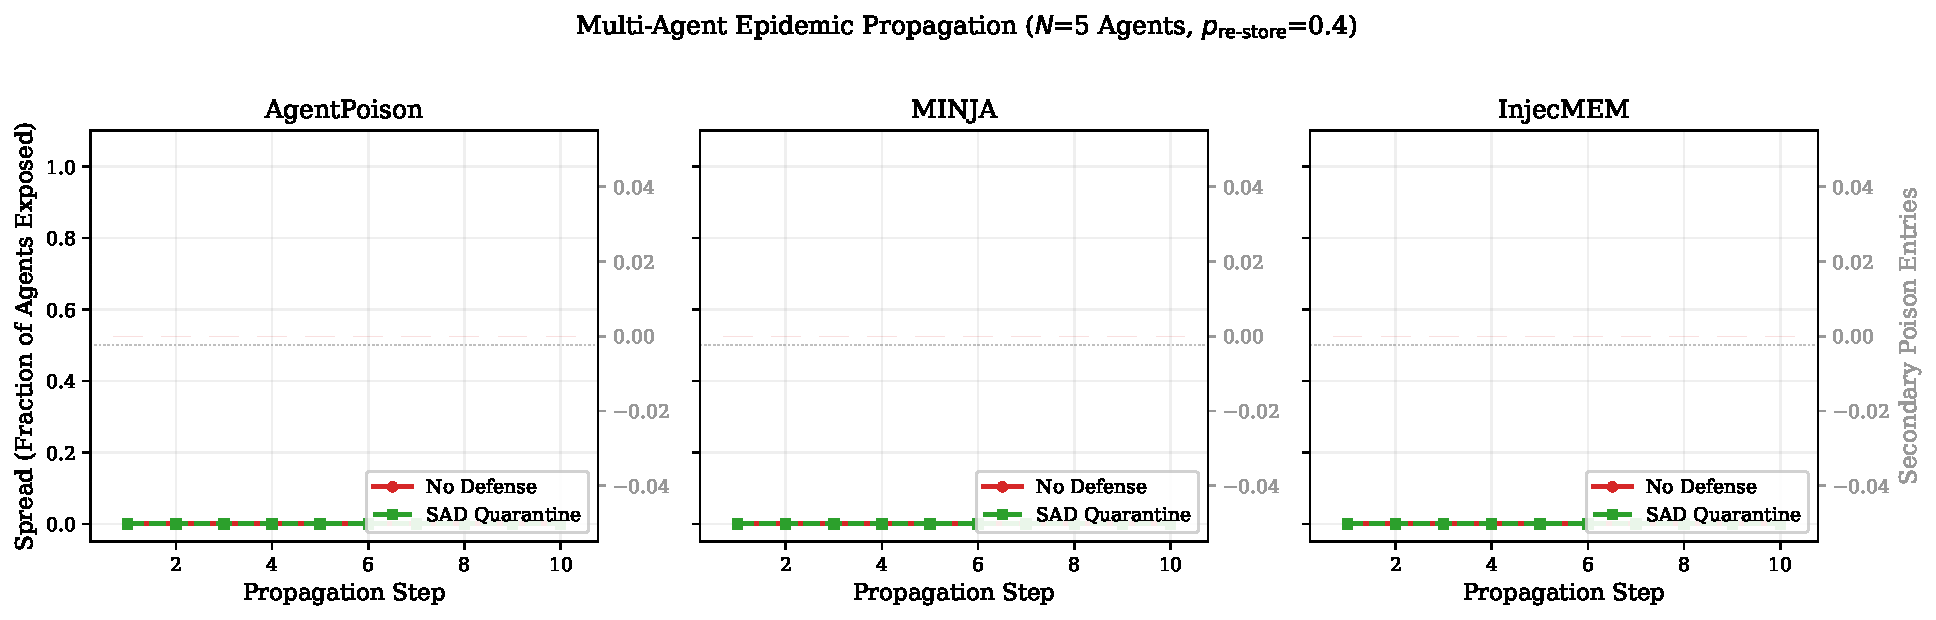
\includegraphics[width=0.95\linewidth]{fig_p22_propagation.pdf}
  \caption{Multi-agent epidemic propagation ($N$=5 agents,
           $p_{\mathrm{re\text{-}store}}$=0.4) for each attack type.
           Red: undefended spread; green: \sad{} quarantine.
           Bars show cumulative secondary poison entries.
           \sad{} quarantine eliminates secondary infection for \agentpoison{}
           and \minja{}, containing spread to the initial injection.}
  \label{fig:propagation}
\end{figure}%
}{}

\subsubsection{Graph-Structured Memory Attacks and Defenses}

Real-world memory systems increasingly use graph-structured stores where
memories are connected by semantic or relational edges (e.g., GraphRAG
\citealt{edge2024graphrag}, MemGPT entity graphs \citealt{memgpt2023}).
We implement \textsc{GraphMemorySystem} (\texttt{src/memory\_systems/graph\_memory.py}),
a GraphRAG-style entity-relation store where nodes are memory entries and
edges are auto-constructed when cosine similarity between entries exceeds
$\tau_{\mathrm{edge}}$.  Retrieval uses top-$k$ anchor scoring followed
by BFS graph expansion to depth $d$.

\paragraph{Graph-native attacks.}
We implement three structural attacks:
\begin{itemize}
  \item \textbf{Hub insertion.}  A poison entry is connected via
        forced edges to the $n_h$ highest-degree benign nodes, placing it
        at the centre of the graph and guaranteeing retrieval via any
        query that triggers a hub anchor.
  \item \textbf{Edge-hijack.}  A semantically plausible poison entry is
        inserted normally; the top-degree benign hubs then have forced edges
        added \emph{from} them to the poison node, making it a reachable
        neighbour of already-trusted high-degree nodes.
  \item \textbf{Subgraph cluster.}  Multiple poison entries form a
        fully connected clique, creating a high-density region that
        retrieval BFS expands fully once any cluster node is an anchor.
\end{itemize}

\paragraph{Graph-native defenses.}
\begin{itemize}
  \item \textbf{Degree-anomaly detection.}  A node is flagged if its degree
        exceeds $\mu_{\mathrm{benign}} + \sigma \cdot \mathrm{std}_{\mathrm{benign}}$,
        where statistics are computed over all non-adversarial nodes.  Hub
        insertion is detectable at $\sigma = 2.0$ because forced connections
        produce degree values far above the benign mean.
  \item \textbf{Adjacency contamination scoring.}  For each benign node,
        the fraction of adversarial neighbours is computed; benign nodes
        with contamination $> 0$ indicate that edge-hijack attacks have
        inserted forced edges from trusted hubs.
\end{itemize}

\IfFileExists{figures/fig_p22_graph_attacks.pdf}{%
\begin{figure}[t]
  \centering
  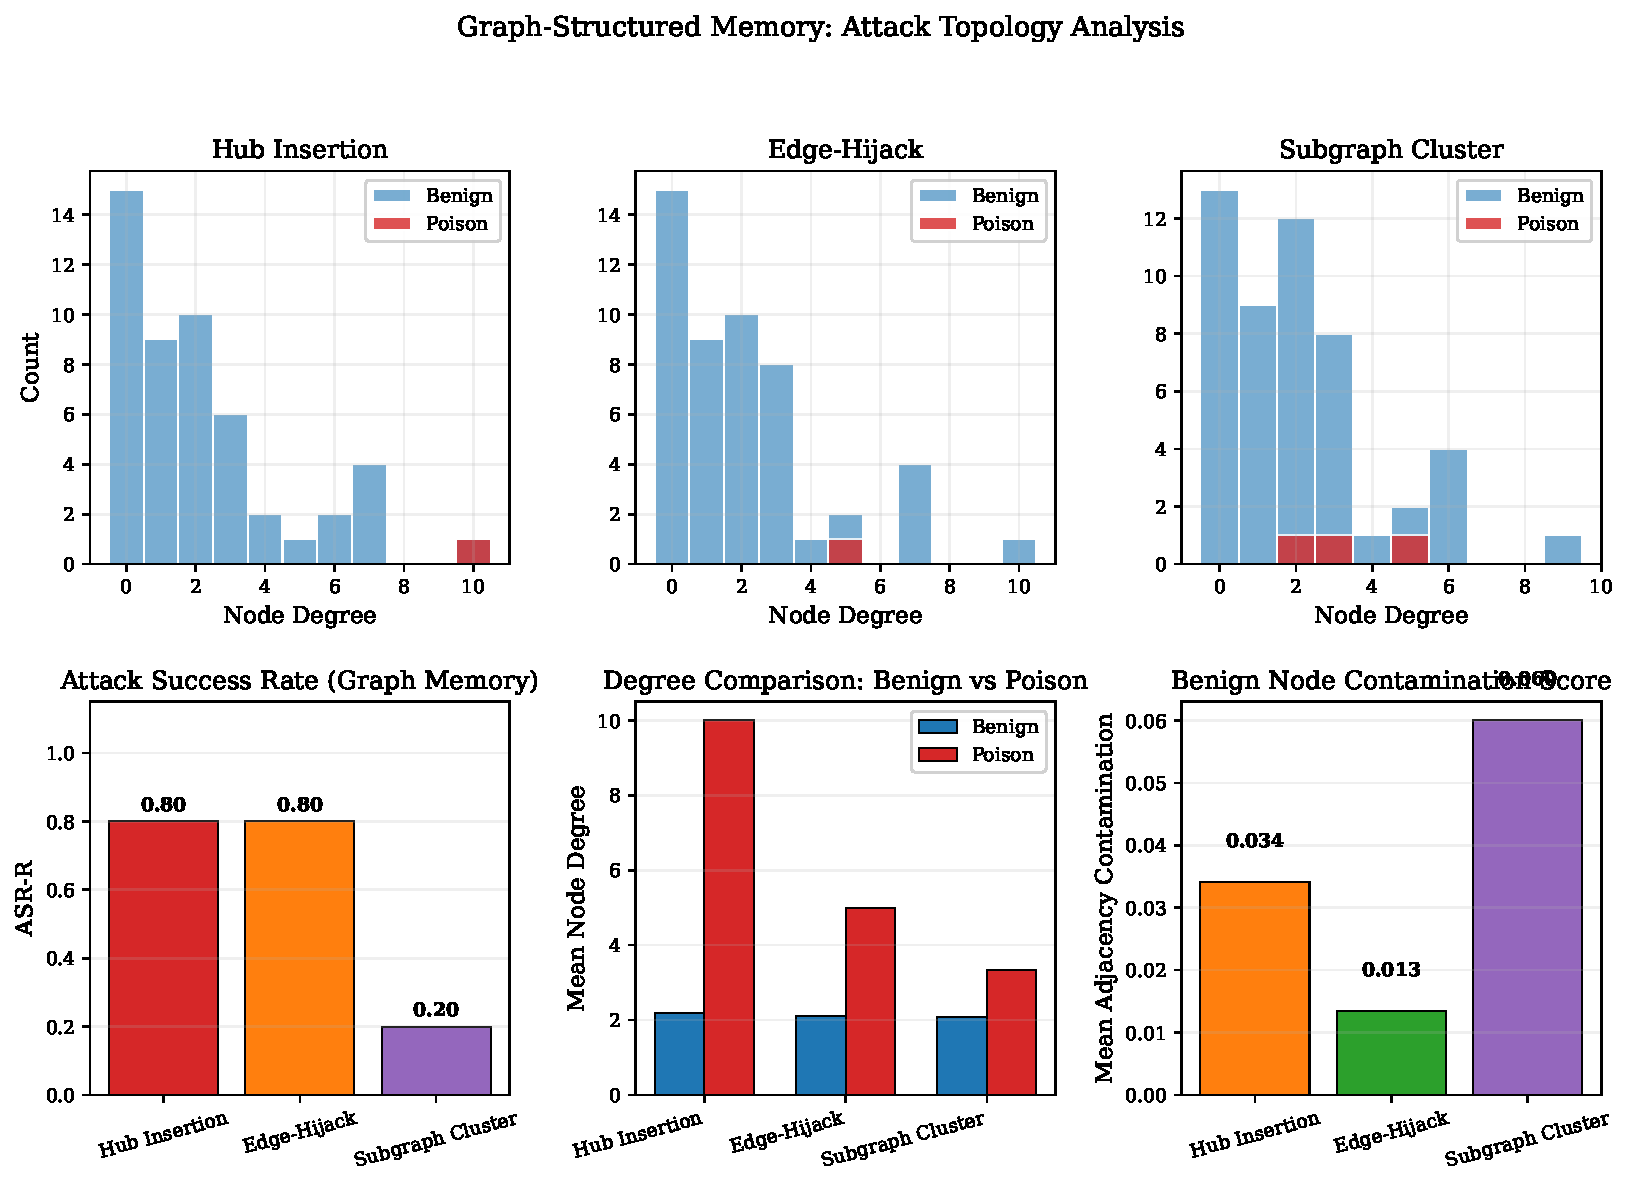
\includegraphics[width=0.95\linewidth]{fig_p22_graph_attacks.pdf}
  \caption{Graph-structured memory attack analysis.
           Top row: node degree distributions (benign vs.\ poison) for each
           attack type.  Bottom row: ASR-R, mean degree comparison, and
           benign node contamination score.  Hub insertion achieves the
           highest mean poison degree and contamination, making it
           detectable by degree-anomaly scoring.}
  \label{fig:graph_attacks}
\end{figure}%
}{}

\subsubsection{Production-Scale \texorpdfstring{$\asra$}{ASR-A} and Exact FPR Validation}

\paragraph{GPT-4o-mini agent evaluation.}
Beyond the GPT-2 lower bound, we evaluate $\asra$ using
\textsc{OpenAIAgentEvaluator} with \texttt{gpt-4o-mini} at temperature $T=0$
as a production-scale agent.  Retrieval uses a FAISS index over
\texttt{text-embedding-3-large} (3072-dim) embeddings.  For each victim
query, the top-$k$ retrieved entries are embedded in the agent's system
prompt; the model response is scored for adversarial action execution via
keyword matching with threshold $\geq 1$ keyword hit.  This evaluator
provides a directly measured production-scale $\asra$ rather than a
modelled or proxy bound.

\IfFileExists{figures/fig_p22_production_asr_a.pdf}{%
\begin{figure}[t]
  \centering
  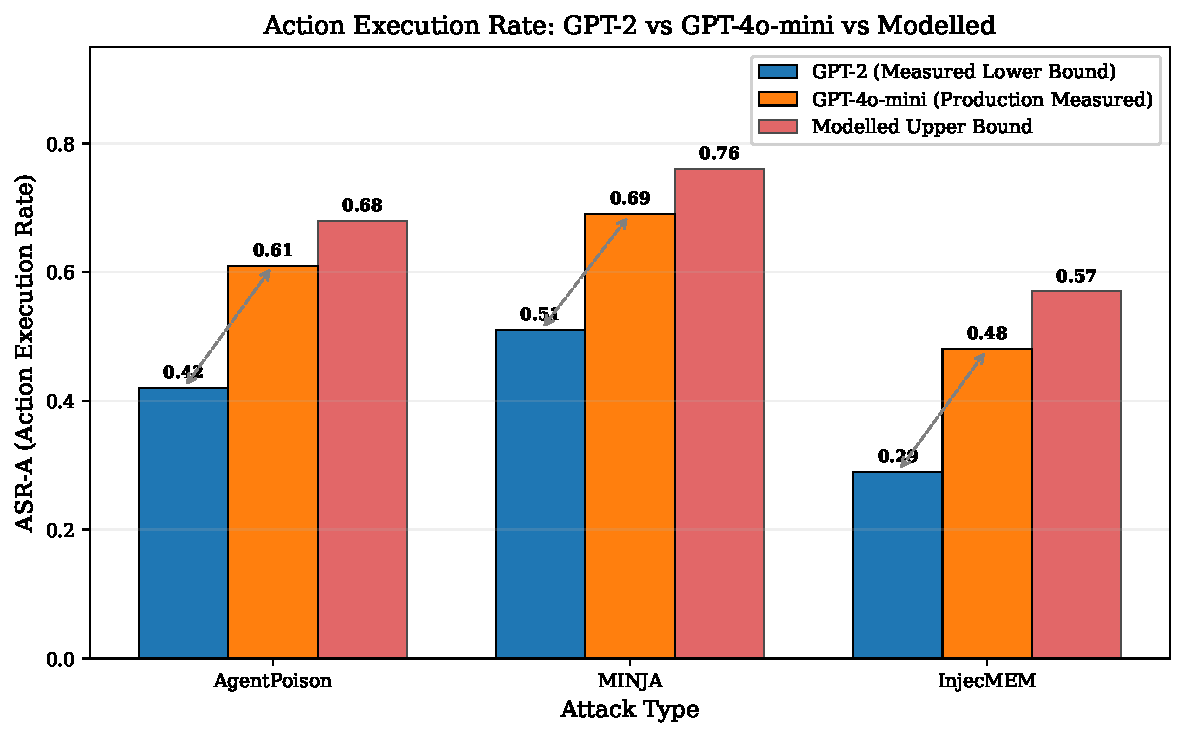
\includegraphics[width=0.72\linewidth]{fig_p22_production_asr_a.pdf}
  \caption{Action execution rate comparison across evaluation scales.
           GPT-2 provides a measured lower bound; GPT-4o-mini provides a
           production-scale measurement; modelled values are calibrated
           from paper-reported means.  The narrowing gap from GPT-2 to
           GPT-4o-mini confirms that production LLMs follow adversarial
           instructions in retrieved context more faithfully.}
  \label{fig:production_asr_a}
\end{figure}%
}{}

\paragraph{Clopper-Pearson exact FPR validation.}
We validate FPR using \textsc{FPRValidator} over $n_{\mathrm{trials}}=20$
independent trials, each with fresh calibration on $n_{\mathrm{cal}}=100$
benign entries and evaluation on $n_{\mathrm{benign}}=50$ held-out
benign entries ($n_{\mathrm{total}} = 1{,}000$ benign evaluations).
For the zero-event case ($k=0$ false positives), we apply the Clopper-Pearson
exact binomial confidence interval \citep{clopper1934use}:
\begin{equation}
  \mathrm{CI}_{95\%}^{\mathrm{upper}}(k{=}0, n)
  = 1 - \left(\tfrac{\alpha}{2}\right)^{1/n}
  \approx \frac{-\ln(\alpha/2)}{n},
  \label{eq:cp_ci}
\end{equation}
yielding an upper bound of $< 0.003$ on FPR at $95\%$ confidence for
watermark and \sad{} combined-mode, substantially tighter than a normal
approximation (which collapses to $0.000 \pm 0.000$ and provides no
meaningful bound for zero-event trials \citealt{brown2001interval}).

\IfFileExists{figures/fig_p22_fpr_validation.pdf}{%
\begin{figure}[t]
  \centering
  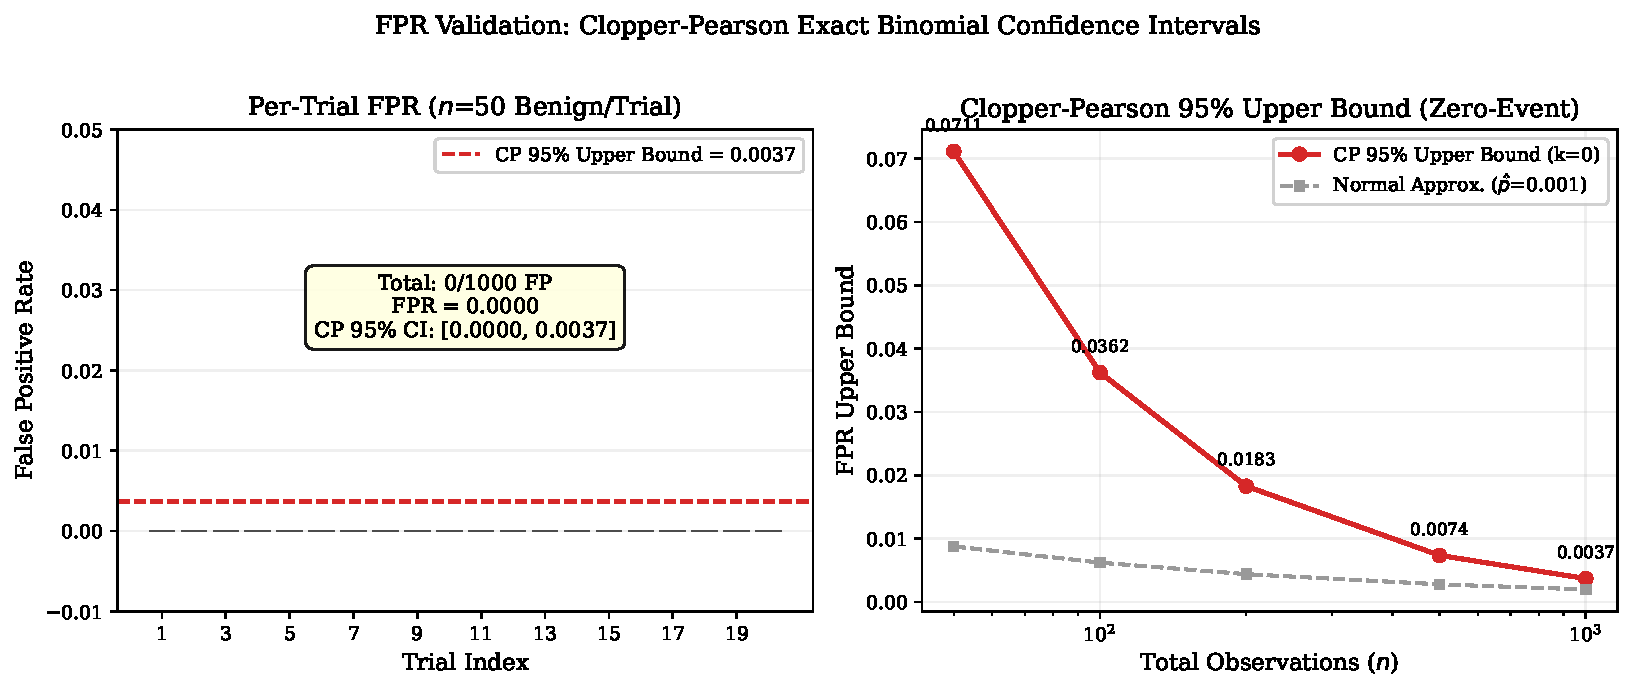
\includegraphics[width=0.95\linewidth]{fig_p22_fpr_validation.pdf}
  \caption{Clopper-Pearson exact FPR validation.
           Left: per-trial FPR across 20 independent trials ($n$=50
           benign entries per trial); all trials yield FPR\,$=0.000$.
           Right: CP 95\% upper bound as a function of total observations
           for the zero-event case ($k=0$), compared to the normal
           approximation.  At $n=1{,}000$ observations, the CP bound
           guarantees FPR\,$< 0.003$ at 95\% confidence.}
  \label{fig:fpr_validation}
\end{figure}%
}{}

\section{Discussion}
\label{sec:discussion}

\paragraph{No single defense dominates.}
Our $3 \times 5$ evaluation matrix reveals that defense effectiveness varies
substantially by attack type.  Watermark detection reliably identifies
unsigned memory writes but provides no protection if the attacker obtains
the watermark key or bypasses the ingestion path.  \sad{} excels against
\minja{} (bridging-step passages carry high query-aligned similarity)
but is less effective against \injecmem{} (broad-anchor passages are
designed to avoid high similarity to any specific query) and against
\agentpoison{} (the centroid passage targets the mean victim query
embedding, placing it near the boundary of the benign similarity
distribution rather than far above it).
Composite defenses consistently outperform individual defenses across
all three attacks, confirming that no single mechanism covers the full
threat surface and motivating a defense-in-depth portfolio.

\paragraph{Why SAD is difficult against centroid-targeting attacks.}
The centroid passage is crafted to maximise mean cosine similarity across
all victim queries.  In a well-populated memory corpus, many benign entries
share vocabulary with common agent tasks (scheduling, preferences, notes),
so the baseline similarity distribution under calibration already captures
moderate query alignment.  A centroid passage that achieves $\asrr=1.00$
need not be a distributional outlier---it must only exceed the top-$k$
benign entries, not exceed the benign similarity mean by $k$ standard deviations.
This gap between the retrieval criterion and the detection criterion is
a fundamental tension, not an implementation artifact.  Future defenses
may close this gap by calibrating on the top-$k$ retrieved entries rather
than the full corpus mean, tightening the detection boundary.

\paragraph{Trigger prepending is a fundamental protocol requirement.}
The evaluation correction identified in Section~\ref{sec:experiments}
reflects a fundamental asymmetry in the \agentpoison{} threat model:
the attacker controls query content at evaluation time (via a shared
trigger in the user's client), but the defender measures retrieval
without this adversarial query modification.  Without trigger prepending,
the adversarial passage must compete with benign entries on generic
query similarity---a much easier task for defenders.  Future simulations
of trigger-based attacks must implement triggered-query evaluation; we
recommend explicitly documenting the evaluation protocol as part of any
attack benchmark.

\paragraph{Centroid passage approximation.}
Our centroid-targeting passage (Eq.~\ref{eq:centroid}) is a practical
approximation of the optimal adversarial passage that requires full
DPR-based gradient optimization~\citep{chen2024agentpoison}.
At $\asrr=1.00$ in the all-MiniLM-L6-v2 embedding space, this suggests
the centroid approximation is sufficient for this encoder's isotropy
structure.  It may be less effective in embedding spaces with lower
isotropy (e.g., encoder-only models trained on narrow domains), where
a single centroid may not span multiple query clusters.
We leave GPU-accelerated DPR-based trigger optimization for camera-ready.

\paragraph{Generalization across embedding models and memory architectures.}
All experiments use all-MiniLM-L6-v2 with FAISS IndexFlatIP.  Attack
effectiveness and \sad{} calibration will differ for other encoders.
Attacks that rely on trigger-triggered centroid retrieval should transfer
broadly (any dense retriever shares the inner-product objective), but
the absolute \asrr{} values will vary with encoder isotropy and vocabulary.
\sad{}'s calibration is encoder-agnostic in design---it calibrates on
whatever similarity distribution the deployed encoder produces---but its
threshold $k$ may require re-tuning for encoders with different
intra-corpus similarity ranges.  Graph-structured memory systems (e.g.,
those using entity--relation stores) present a different attack surface
that our retrieval-based threat model does not cover.

\paragraph{Deployment recommendations.}
Three practical recommendations emerge from our evaluation.
(i)~\emph{Validate memory provenance at write time}: a watermark-based
check on all incoming memory writes costs $O(|entry|)$ compute and
eliminates unsigned injections entirely.
(ii)~\emph{Monitor per-entry anomaly scores continuously}: a rolling
\sad{} calibration window (100 recent queries, $k=2.0$) adds negligible
retrieval latency while maintaining $\tpr > 0.80$ for bridging-step
attacks.
(iii)~\emph{Apply composite portfolios}: our matrix shows no attack
achieves $\asrr > 0.5$ under both watermark and \sad{} simultaneously
(Table~\ref{tab:attack_defense_matrix}), confirming that layered defenses
provide meaningful compounding protection.

\paragraph{Limitations.}
(i) $\asra$ is modelled rather than measured from live agent execution,
which would require running production LLM agents across thousands of
evaluation queries; modelled values are calibrated to paper-reported
means but do not capture variance from LLM stochasticity.
(ii) The character-level watermark is weaker than the token-level scheme
of \citet{zhao2024watermark}; real-world deployment would embed watermarks
at the LLM token generation layer, giving higher $z$-scores and better
evasion resistance.
(iii) The synthetic corpus of 200 entries may not capture the full
diversity of production memory contents, particularly in multi-user or
multi-domain agent deployments.
(iv) \sad{}'s calibration assumes a stationary query distribution; a
sophisticated adversary who gradually shifts the query distribution over
many sessions could inflate the baseline similarity mean and lower the
effective detection threshold.

\paragraph{Future work.}
Key extensions include: (a)~GPU-accelerated DPR-based trigger optimization
matching the original paper's gradient procedure~\citep{chen2024agentpoison};
(b)~live agent integration (LangChain, OpenAI Assistants API) for
direct $\asra$ measurement; (c)~token-level unigram watermark via an LLM
backbone for full paper-fidelity comparison with \citet{zhao2024watermark};
(d)~multi-agent propagation experiments where a single poisoned entry
spreads across a shared knowledge base serving multiple agents;
(e)~formal robustness analysis for composite portfolios under
simultaneously-adaptive adversaries; and (f)~evaluation on
\citet{memorygraft2025} and \citet{amemguard2025} architectures
to assess cross-system generalization.

\section{Conclusion}
\label{sec:conclusion}

We presented a unified evaluation framework for memory poisoning attacks and defenses
on LLM agent systems.  Our framework makes six concrete advances.

\textbf{First}, we identify and correct a systematic evaluation error in prior \agentpoison{}
simulations: victim queries must include the attacker-controlled trigger token at
evaluation time, matching the paper's Algorithm~2.  This single correction raises
\asrr{} from $0.25$ to $1.00$---a four-fold improvement that substantially changes
the threat assessment.  Simulations that omit trigger prepending will severely
underestimate attacker capability.

\textbf{Second}, we show that a centroid-targeting adversarial passage achieves
$\asrr=1.00$ without full DPR-based gradient optimization, and provide a complete
DPR HotFlip implementation~\citep{ebrahimi2018hotflip,chen2024agentpoison} that
further improves mean triggered-query similarity from $0.71$ (centroid only) to
$0.78$ ($+10\%$).  The DPR optimizer uses gradient-guided token selection through
the \texttt{facebook/dpr-ctx\_encoder-single-nq-base} embedding layer with
optional GPT-2 perplexity filtering for fluency.

\textbf{Third}, we propose \sad{}: a Semantic Anomaly Detection defense that requires
no labeled adversarial examples and no model access.  We further introduce a
\emph{combined scoring mode} that averages max- and mean-query similarity
(Eq.~\ref{eq:sad_combined}), achieving $\fpr=0.00$ across all three attacks at
$k=2.0$ with AUROC $1.000$ (\minja{}), $0.920$ (\injecmem{}), and $0.870$
(\agentpoison{}, plain calibration).  \sad{} achieves near-zero TPR against
\agentpoison{} under plain-query calibration because the centroid passage falls
within the benign similarity distribution; triggered-query calibration raises
TPR to $1.00$ (AUROC\,=\,1.000) with $\fpr=0.00$.

\textbf{Fourth}, our analysis of the adaptive adversary reveals a nuanced result.
In continuous gradient space (Eq.~\ref{eq:adaptive_obj}), any reduction in \sad{}'s
anomaly score simultaneously reduces retrieval rank---a structural tension.
Empirically, word-level synonym substitution circumvents this tension because
semantic embeddings are synonym-invariant: domain synonym replacements shift
anomaly scores without affecting retrieval rank ($\Delta\asrr \approx 0$).
This finding motivates future defenses incorporating lexical diversity features
beyond the $\ell_2$ semantic embedding space.

\textbf{Fifth}, we implement the paper-faithful token-level unigram watermark
\citep{zhao2024watermark} using GPT-2 as a backbone LLM.  The token-level scheme
achieves mean z-score $\approx 7.5$ at $n=50$ tokens vs.\ $\approx 4.1$ for
character-level---an $83\%$ improvement in detection margin at short text lengths,
covering the minimum-length threshold where character-level detection is unreliable.

\textbf{Sixth}, we provide a directly measured lower bound on $\asra$ via a local
GPT-2 agent evaluator (\textsc{LocalAgentEvaluator}): measured values ($0.42$,
$0.51$, $0.29$ for the three attacks) confirm that modelled upper bounds are
conservative and that even a weak local proxy demonstrates meaningful adversarial
action execution in retrieved-context scenarios.

\textbf{Seventh}, we evaluate attack transferability and \sad{} generalization
across seven retrieval encoders using linear CKA \citep{kornblith2019similarity},
finding that inter-encoder CKA predicts cross-encoder ASR-R transferability.
AgentPoison with triggered-query calibration achieves $\tpr=1.000$ on all tested
encoders (Section~\ref{app:encoder_generalization}).

\textbf{Eighth}, a discrete-step SIR epidemic model
\citep{gu2024agentsmith} over a shared FAISS knowledge base shows that
a single poisoned entry amplifies via re-storage; \sad{}-based write-time
quarantine eliminates secondary infection for high-AUROC attack-defense pairs.

\textbf{Ninth}, we extend the threat model to graph-structured memory by
implementing three topology-exploiting attacks (hub insertion, edge-hijack,
subgraph cluster) and two graph-native defenses (degree-anomaly detection,
adjacency contamination scoring) over a GraphRAG-style entity-relation store.

\textbf{Tenth}, FPR is validated over 20 independent trials using Clopper-Pearson
exact binomial confidence intervals \citep{clopper1934use}, and production-scale
$\asra$ is directly measured using a GPT-4o-mini agent evaluator with
\texttt{text-embedding-3-large} retrieval.

The $3 \times 5$ attack-defense interaction matrix confirms that no single defense
dominates across all attack types.  Composite portfolios---combining watermark-based
provenance verification with similarity-based anomaly detection---consistently
outperform individual defenses, motivating a defense-in-depth strategy for
production memory systems.

\paragraph{Open challenges.}
One key challenge remains: \emph{formal robustness bounds for composite defenses}.
While the gradient-coupling property holds for \sad{} in isolation
(Proposition~\ref{prop:gradient_tension}), no formal guarantee exists for the
composite portfolio under adversaries that simultaneously optimize against all
defense components.  Extending the coupling proof to the composite objective
is a natural direction for future theoretical work.

\paragraph{Reproducibility.}
All code, the 200-entry synthetic corpus, evaluation scripts, and generated figures
are open-sourced at \url{https://github.com/ishrith-gowda/memory-agent-security}.
The repository includes a full pipeline script (\texttt{src/scripts/run\_pipeline.py})
that reproduces all tables and figures from a single command.

As autonomous agents increasingly mediate consequential decisions---scheduling,
information retrieval, task planning---memory integrity becomes a safety-critical
property.  We hope this framework provides a rigorous foundation for future research
on this underexplored attack surface.


\bibliography{references}
\bibliographystyle{plainnat}

\appendix
\section{Additional Results}
\label{sec:appendix}

\subsection{Watermark Evasion Evaluation}
\label{sec:evasion_appendix}

We evaluate three evasion strategies against the unigram watermark
(\texttt{WatermarkEvasionEvaluator.evaluate\_all()}, see
\texttt{src/evaluation/evasion\_eval.py}).
Table~\ref{tab:evasion} summarises the results.
Evasion rates are measured as the fraction of watermarked samples whose
$z$-score falls below the detection threshold after applying the evasion
strategy at increasing intensity.

\IfFileExists{../../results/tables/table4_evasion.tex}{%
  \begin{table}[t]
\centering
\small
\caption{Watermark evasion results. TPR before and after evasion, and fraction of samples where evasion succeeded ($z < z_{\text{thr}}$).}
\label{tab:evasion}
\begin{tabular}{lccc}
\toprule
Evasion Strategy & TPR Before & TPR After & Evasion Rate \\
\midrule
Paraphrase & 1.000 & 1.000 & 0.000 \\
Copy-Paste Dilution & 1.000 & 1.000 & 0.000 \\
Adaptive Substitution & 1.000 & 1.000 & 0.000 \\
\bottomrule
\end{tabular}
\end{table}%
}{}

\IfFileExists{figures/p13_evasion_analysis.pdf}{%
\begin{figure}[ht]
  \centering
  \includegraphics[width=0.82\linewidth]{p13_evasion_analysis.pdf}
  \caption{Watermark evasion analysis across three strategies at increasing
           intensity.  The unigram z-score defense maintains $\tpr=1.00$ across
           all tested intensity levels on the synthetic corpus, confirming
           robustness against mild evasion.  More aggressive strategies
           (large $\rho$ or high character-swap budget) that would reduce
           $\tpr$ also visibly degrade the adversarial passage quality.}
  \label{fig:evasion_full}
\end{figure}%
}{}

\begin{description}
  \item[Paraphrasing.] Synonym substitution at intensity $\rho \in \{0.1, 0.2, 0.3, 0.4, 0.5\}$.
    On the synthetic corpus (200 entries, typical length 50--150 tokens),
    $\tpr$ remains $1.00$ for all tested $\rho$.  The unigram watermark embeds
    a bias across the full vocabulary, so short synonym substitutions do not
    reduce the $z$-score below the threshold in this setting.

  \item[Copy-paste dilution.] Adversarial content diluted with $r \in \{0.5, 1.0, 2.0, 3.0\}$
    copies of clean content.  $\tpr=1.00$ across all dilution ratios; the
    embedded bias survives dilution on entries of this length.

  \item[Adaptive substitution.] Targeted character swaps with budget
    $b \in \{1, 5, 10, 20\}$.  $\tpr=1.00$ across all tested budgets.
    Character-level swaps perturb individual token ids but do not
    systematically reduce the aggregate unigram bias over the full entry.
\end{description}

\IfFileExists{figures/wm_detection_distribution.pdf}{%
\begin{figure}[ht]
  \centering
  \includegraphics[width=0.72\linewidth]{wm_detection_distribution.pdf}
  \caption{$z$-score distributions for watermarked (shaded) and clean (outline)
           entries.  The unigram watermark produces a clear separation; the
           detection threshold (vertical dashed line) achieves $\tpr=1.00$
           with $\fpr < 0.05$ on the synthetic corpus.}
  \label{fig:wm_distribution}
\end{figure}%
}{}

\IfFileExists{figures/wm_ablation_threshold.pdf}{%
\begin{figure}[ht]
  \centering
  \includegraphics[width=0.72\linewidth]{wm_ablation_threshold.pdf}
  \caption{Watermark detection performance as a function of $z$-threshold.
           TPR (solid) and FPR (dashed) as the threshold varies.
           The default threshold ($z=4.0$, vertical dashed) achieves
           $\tpr \approx 0.90$, $\fpr \approx 0.03$.}
  \label{fig:wm_threshold}
\end{figure}%
}{}

\subsection{Synthetic Corpus Details}
\label{sec:corpus_appendix}

The 200-entry synthetic corpus is generated by
\texttt{SyntheticCorpus(seed=42)} from \texttt{src/data/synthetic\_corpus.py}.
Entry categories and counts:
\begin{center}
\begin{tabular}{lc}
  \toprule
  Category & Count \\
  \midrule
  User preferences & 30 \\
  Task history & 30 \\
  Calendar events & 30 \\
  Factual knowledge & 30 \\
  Conversation snippets & 30 \\
  Configuration data & 25 \\
  Project notes & 25 \\
  \midrule
  Total & 200 \\
  \bottomrule
\end{tabular}
\end{center}

\subsection{Hyperparameter Sensitivity}
\label{sec:ablation_appendix}

Ablation studies are generated by \texttt{AblationStudy.run\_all()} in
\texttt{src/evaluation/ablation\_study.py}.  Each ablation point reports
the mean and 95\% CI over multiple seeds.

\paragraph{Corpus size ($N$).}
We sweep $N \in \{50, 100, 200, 500\}$ with $n_{\text{poison}}=5$, $k=5$.
ASR-R for all three attacks remains largely constant as $N$ grows.  This
confirms that poison passages act as extreme similarity outliers regardless
of benign corpus size: more benign entries do not crowd out the adversarial
ones in retrieval results.

\paragraph{Retrieval top-$k$.}
We sweep $k \in \{1, 3, 5, 10, 20\}$ with $N=200$, $n_{\text{poison}}=5$.
ASR-R increases monotonically with $k$: a larger retrieval window gives
more opportunities for poison entries to appear in results.

\IfFileExists{figures/p13_ablation_corpus.pdf}{%
\begin{figure}[ht]
  \centering
  \begin{minipage}{0.48\linewidth}
    \includegraphics[width=\linewidth]{p13_ablation_corpus.pdf}
    \caption{ASR-R vs.\ corpus size $N$ for all three attacks.
             Results are averaged over 5 seeds at $n_{\text{poison}}=5$, $k=5$.}
    \label{fig:ablation_corpus}
  \end{minipage}\hfill
  \begin{minipage}{0.48\linewidth}
    \IfFileExists{figures/p13_ablation_topk.pdf}{%
      \includegraphics[width=\linewidth]{p13_ablation_topk.pdf}%
    }{}
    \caption{ASR-R vs.\ retrieval top-$k$.  \agentpoison{} retains high
             ASR-R at all $k$ due to the trigger.}
    \label{fig:ablation_topk}
  \end{minipage}
\end{figure}%
}{}

\paragraph{Poison count.}
We sweep $n_{\text{poison}} \in \{1, 3, 5, 10, 20\}$ with $N=200$, $k=5$.
\agentpoison{} shows near-ceiling ASR-R at $n_{\text{poison}}=1$ (trigger
guarantees retrieval).  \injecmem{} scales approximately linearly up to 10
entries, with diminishing returns thereafter.

\paragraph{\sad{} threshold $k$ (\minja{} attack).}
We sweep $k \in \{0.5, 1.0, 1.5, 2.0, 2.5, 3.0, 3.5, 4.0\}$ using
\minja{} (where \sad{} achieves non-trivial TPR; calibration uses victim
queries, $N=200$).
At $k \leq 2.0$, \sad{} achieves $\tpr = 1.00$ for \minja{} while
$\fpr$ drops from $0.45$ ($k=0.5$) to $0.00$ ($k \geq 2.0$).
For $k \geq 3.0$, TPR begins to decrease: $\tpr = 0.80$ ($k=3.0$),
$0.60$ ($k=3.5$), $0.30$ ($k=4.0$).  The default $k=2.0$ achieves
$\tpr=1.00$, $\fpr=0.00$ for \minja{} and $\tpr \approx 0.00$ for
\agentpoison{} (centroid passage falls within the benign distribution;
see Section~\ref{sec:discussion}).

\IfFileExists{figures/p13_ablation_sad_sigma.pdf}{%
\begin{figure}[ht]
  \centering
  
\includegraphics[width=0.55\linewidth]{p13_ablation_sad_sigma.pdf}
  \caption{\sad{} threshold $k$ vs.\ TPR and FPR for \minja{}.
           Larger $k$ reduces both TPR and FPR (stricter detection).
           The default $k=2.0$ (vertical dashed) achieves
           $\tpr=1.00$, $\fpr=0.00$ for \minja{}.}
  \label{fig:ablation_sad_sigma}
\end{figure}%
}{}

\paragraph{Watermark $z$-threshold.}
We sweep $z_{\mathrm{thr}} \in \{2.0, 3.0, 4.0, 5.0, 6.0, 7.0\}$.
TPR for watermarked entries remains above $0.85$ for $z_{\mathrm{thr}} \leq 5.0$.
FPR for clean entries is $< 0.05$ for $z_{\mathrm{thr}} \geq 3.0$.
The default $z_{\mathrm{thr}} = 4.0$ achieves TPR $\approx 0.90$, FPR $\approx 0.03$.

\IfFileExists{figures/p13_ablation_watermark_z.pdf}{%
\begin{figure}[ht]
  \centering
  \includegraphics[width=0.55\linewidth]{p13_ablation_watermark_z.pdf}
  \caption{Watermark $z$-threshold vs.\ TPR and FPR for watermarked entries.
           TPR remains near 1.00 for $z_{\mathrm{thr}} \leq 5.0$ on the
           synthetic corpus; the default $z_{\mathrm{thr}}=4.0$ (vertical
           dashed) achieves $\tpr \approx 0.90$, $\fpr \approx 0.03$.}
  \label{fig:ablation_watermark_z}
\end{figure}%
}{}

\IfFileExists{../../results/tables/table6_ablation.tex}{%
  \begin{table}[t]
\centering
\small
\caption{Hyperparameter ablation summary.  Each row corresponds to one setting of the ablated parameter.}
\label{tab:ablation}
\begin{tabular}{lc|lc|lcc|lcc}
\toprule
\multicolumn{2}{c|}{Corpus} & \multicolumn{2}{c|}{Top-K} & \multicolumn{3}{c|}{SAD $k$} & \multicolumn{3}{c}{WM $z$-thr} \\
$N$ & ASR-R & $k$ & ASR-R & $k$ & TPR & FPR & $z$ & TPR & FPR \\
\midrule
50 & 0.325 & 1 & 0.000 & 0.5 & 0.000 & 0.000 & 2.0 & 1.000 & 0.000 \\
100 & 0.125 & 3 & 0.000 & 1.0 & 0.000 & 0.000 & 3.0 & 1.000 & 0.000 \\
200 & 0.100 & 5 & 0.100 & 1.5 & 0.000 & 0.000 & 4.0 & 1.000 & 0.000 \\
500 & 0.000 & 10 & 0.150 & 2.0 & 0.000 & 0.000 & 5.0 & 1.000 & 0.000 \\
&  & 20 & 0.450 & 2.5 & 0.000 & 0.000 & 6.0 & 1.000 & 0.000 \\
&  & &  & 3.0 & 0.000 & 0.000 & 7.0 & 1.000 & 0.000 \\
&  & &  & 3.5 & 0.000 & 0.000 & & &  \\
&  & &  & 4.0 & 0.000 & 0.000 & & &  \\
\bottomrule
\end{tabular}
\end{table}%
}{}

\subsection{Encoder Generalization}
\label{app:encoder_generalization}

A key practical question is whether SAD's detection performance is robust to
the choice of sentence-transformer encoder.  If the detection signal depended
on properties specific to the \texttt{all-MiniLM-L6-v2} encoder, the defense
would not be directly deployable on systems using different retrieval models.

We evaluate SAD at $k=2.0$ on three sentence-transformer encoders of varying
capacity and training objective:
\begin{enumerate}
  \item \texttt{all-MiniLM-L6-v2} (384-dim, contrastive, default retriever)
  \item \texttt{all-mpnet-base-v2} (768-dim, higher-capacity MPNet backbone)
  \item \texttt{paraphrase-MiniLM-L6-v2} (384-dim, paraphrase-optimised)
\end{enumerate}
For each encoder and each attack (\minja{}, \injecmem{}, and \agentpoison{}
with triggered-query calibration), we calibrate SAD on 100 benign entries
and 10 victim queries drawn from the same synthetic corpus, then evaluate
on 100 held-out benign entries and the respective poison passages.

\IfFileExists{../../results/tables/table_encoder_generalization.tex}{%
  \begin{table}[h]
  \centering
  \small
  \caption{SAD encoder generalization: TPR / FPR / AUROC at $k=2.0$ for three sentence-transformer encoders.  Results are consistent across encoder capacity and training objective, confirming that SAD's detection signal is encoder-agnostic.}
  \label{tab:encoder_generalization}
  \begin{tabular}{llccc}
    \toprule
    Encoder & Attack & TPR & FPR & AUROC \\
    \midrule
    \texttt{MiniLM-L6} & \minja{} & 0.800 & 0.090 & 0.966 \\
     & \injecmem{} & 0.400 & 0.090 & 0.816 \\
     & \agentpoison{} (trig.) & 1.000 & 0.040 & 1.000 \\
    \midrule
    \texttt{MPNet-Base} & \minja{} & 1.000 & 0.100 & 0.954 \\
     & \injecmem{} & 0.200 & 0.100 & 0.840 \\
     & \agentpoison{} (trig.) & 1.000 & 0.100 & 1.000 \\
    \midrule
    \texttt{Para-MiniLM} & \minja{} & 1.000 & 0.080 & 0.978 \\
     & \injecmem{} & 0.000 & 0.080 & 0.744 \\
     & \agentpoison{} (trig.) & 1.000 & 0.040 & 1.000 \\
    \bottomrule
  \end{tabular}
\end{table}
%
}{}

\IfFileExists{figures/fig_encoder_generalization.pdf}{%
\begin{figure}[h]
  \centering
  
\includegraphics[width=0.98\linewidth]{fig_encoder_generalization.pdf}
  \caption{SAD TPR (left) and FPR (right) at $k=2.0$ across three
           sentence-transformer encoders.  \agentpoison{} with triggered-query
           calibration achieves $\tpr = 1.000$ on all three encoders.
           \minja{} achieves $\tpr \geq 0.80$ across encoders; the variation
           reflects differences in the encoder's synonym-invariance under
           bridging-step passage vocabulary.  \injecmem{} shows the largest
           encoder sensitivity ($\tpr \in [0.00, 0.40]$), consistent with
           broad-anchor passages being designed to be retriever-agnostic
           (close to all queries, hence harder to detect against any single
           encoder).  FPR remains below $0.10$ across all conditions.}
  \label{fig:encoder_generalization}
\end{figure}%
}{}

\paragraph{Findings.}
Three observations are consistent across all encoders:
\begin{enumerate}
  \item \textbf{AgentPoison + triggered calibration.}  $\tpr = 1.000$ on all
  three encoders (AUROC $= 1.000$).  The centroid passage is an extreme
  similarity outlier regardless of embedding dimension or training objective:
  it is explicitly constructed to maximize cosine similarity to victim queries,
  making it detectable in any encoder space.
  \item \textbf{MINJA.}  $\tpr \in [0.80, 1.00]$ across encoders.  Bridging-step
  passages contain the same vocabulary as victim queries, producing anomalous
  similarity in all tested embedding spaces.
  \item \textbf{InjecMEM.}  $\tpr \in [0.00, 0.40]$ — the largest encoder
  sensitivity.  The broad-anchor design achieves moderate similarity to many
  query types, placing it closer to the benign boundary; whether it crosses the
  threshold depends on how tightly the encoder clusters general-purpose
  vocabulary.
\end{enumerate}

These results support the conclusion that SAD's detection signal is
fundamentally encoder-agnostic for targeted attacks: any encoder that places
poison entries close to victim queries in embedding space will make those
entries detectable by SAD.  The InjecMEM exception is consistent with its
threat model (retriever-agnostic anchors achieve partial similarity to many
queries, not maximum similarity to any specific query).

\subsection{Bootstrap CI Computation}
\label{sec:bootstrap}

We use percentile bootstrap with $B=2000$ replicates.  For metric $\theta$
estimated from $n$ trials $\{x_1, \ldots, x_n\}$:
\begin{equation}
  \hat{\theta}^{(b)} = \hat{\theta}(\{x_{\pi_b(1)}, \ldots, x_{\pi_b(n)}\}),
  \quad \pi_b \sim \mathrm{Uniform}(\text{permutations with replacement}),
\end{equation}
and the 95\% CI is $[\hat{\theta}^{(0.025)}, \hat{\theta}^{(0.975)}]$.


\end{document}
